% Licence:  Creative Commons Attribution (CC BY 4.0)
% Author: Tim Träris (2022)
% Author: Valentin Weber (2023)
\documentclass{hfubook} % remove `english` for german language

\usepackage{comment} % for multiline comments

\begin{document}

\author{Aljosha Vieth}
\matriculationnumber{271401}
\studyprogram{Informatik}
\streetname{Zollernstraße 87}
\postalcode{75328}
\city{Schömberg}
\email{mail@aljoshavieth.de}
\title{Redis im OLAP Umfeld}
\subtitle{Ist Redis im OLAP Umfeld nützlich?}     % optional
\type{Master Thesis}
\supervisor{Prof. Dr. Piepmeyer}
\cosupervisor{Dr. Weininger}
\date{30.11.2023}

\maketitle

% Roman numbering
\frontmatter
\pagenumbering{Roman}

\chapter*{Abstract\markboth{Abstract}}
\addcontentsline{toc}{chapter}{Abstract}

\section{Englisch}
Redis is a popular NoSQL database that is frequently used in OLTP applications. Nevertheless, there is limited research on using Redis as stand-alone OLAP software. This thesis analyses whether and how Redis can be used as a stand-alone OLAP application. The data and queries of the Star Schema Benchmark (SSB) are used to compare the performance of Redis and PostgreSQL. Various implementation strategies for the SSB in Redis are analysed and compared. It is shown that Redis can process most SSB queries faster than PostgreSQL with the help of the RediSearch module and denormalised and indexed data. However, Redis requires significantly more memory and data customisation, which can have an impact on costs.

\section{Deutsch}
Redis ist eine populäre NoSQL-Datenbank, die häufig in OLTP-Anwendungen eingesetzt wird. Bislang gibt es jedoch wenig Forschung über den Einsatz von Redis in OLAP-Anwendungen. Diese Arbeit untersucht, ob und wie Redis als eigenständige OLAP-Anwendung genutzt werden kann. Dabei wird mithilfe der Daten und Queries des Star Schema Benchmarks (SSB) ein Vergleich der Leistungsfähigkeit zwischen Redis und PostgreSQL erstellt. Es werden verschiedene Implementierungsstrategien für den SSB in Redis betrachtet und verglichen. Dabei zeigt sich, dass Redis mit Hilfe des Moduls RediSearch und denormalisierten und indizierten Daten die meisten SSB-Anfragen schneller verarbeiten kann als PostgreSQL. Allerdings benötigt Redis deutlich mehr Speicher und eine Anpassung der Daten, was sich auf die Kosten auswirken kann.            % Abstract
\tableofcontents                        % Contents
\listoffigures                          % List of Figures
\listoftables                           % List of Tables
\lstlistoflistings                      % List of Code Listings
\abbrtitle
\begin{acronym}[HFU  ] % [HFU  ] controls the width in the list of abbreviations, replace this with your longest acronym
    \acro{HFU}{Hochschule Furtwangen University}
    \acro{SSB}{Star Schema Benchmark}
    \acro{OLAP}{On-Line Analytical Processing}
\end{acronym}
       % Abbreviations

% Content
\mainmatter
\chapter{Einleitung}
\section{Einsatz von Künstlicher Intelligenz} % TODO: Richtigen Platz für diesen Disclaimer finden
Zum Schreiben dieser Arbeit wurde Künstliche Intelligenz (KI) eingesetzt.
Dabei wurden die Tools \enquote{ChatGPT} (GPT-4)~\cite{openai_chatgpt_nodate} der Firma \emph{OpenAI} sowie \enquote{DeepL Write}~\cite{deepl_se_deepl_nodate} von \emph{DeepL SE} verwendet.

\emph{ChatGPT} wurde genutzt, um aus den eigens verfassten Sätzen oder Stichpunkten des Autors ausführlichere Texte zu generieren.
Zusätzlich kam \emph{DeepL Write} zum Einsatz, um die Texte weiter zu verfeinern und ihnen einen akademischen Schreibstil zu verleihen.

KI wurde nicht verwendet, um selbstständig komplette Texte zu formulieren oder neue Informationen zu generieren.
Stattdessen wurden ausschließlich die vom Autor bereitgestellten Informationen verwendet, ohne dass die KI zusätzliche Inhalte oder Änderungen einbrachte.
Etwaige zusätzliche Informationen oder Änderungen, die von der KI vorgeschlagen wurden, fanden keine Berücksichtigung.
Diese Vorgehensweise sorgt dafür, dass die Integrität und Authentizität der Arbeit des Autors unbeeinträchtigt bleiben.

Bei der Entwicklung des praktischen Teils dieser Arbeit wurde \emph{ChatGPT} genutzt, um den selbst geschriebenen Code zu optimieren, zu kommentieren, Beispieldaten zu generieren und Fehler zu analysieren.
\section{Hintergrund und Kontext}
\section{Problemstellung}
\section{Forschungsziel}
\section{Gliederung der Arbeit}
\section{Verwandte Arbeit}

 
% TODO: FIX LATEX ERRORS
\chapter{Technische Grundlagen}
\section{Beliebtheit von Technologien}
% Hier durch bessere Quelle austauschen
In der vorliegenden Arbeit wird die Popularität von bestimmten Technologien auf Basis zweier Indizes dargestellt: dem \emph{\acf{PYPL}}~\cite{carbonnelle_pypl_2023} sowie dem \emph{\acf{TOPDB}}~\cite{carbonnelle_topdb_2023}.  Diese Indizes dienen der Einschätzung der Beliebtheit von Programmiersprachen und Datenbanken und basieren hierbei auf der Häufigkeit von Google-Suchen.

Der \emph{\acf{PYPL}} misst die Beliebtheit von Programmiersprachen anhand der Analyse der Häufigkeit von Suchanfragen nach Tutorials auf Google. 
Dieser Index beruht auf der Annahme, dass eine höhere Anzahl von Suchanfragen nach Tutorials für eine bestimmte Sprache auf eine größere Beliebtheit dieser Sprache hinweist.

Der \emph{\acf{PYPL}} bewertet die Beliebtheit von Datenbanken anhand der Analyse der Suchhäufigkeit nach ihren Namen auf Google.  Eine erhöhte Suchfrequenz nach einer bestimmten Datenbank deutet dabei auf eine größere Popularität hin, ähnlich dem \emph{PYPL}-Index.

\section{\acf{OLAP}}
Viele Unternehmen verwenden heute große Mengen an Geschäftsdaten für eine strategische Planung.
Durch eine Analyse der Daten lassen sich Handlungsempfehlungen ableiten.
Typische Analysen umfassen die Berechnung des Umsatzes einer Filiale innerhalb des letzten Jahres sowie der Vergleich zu vorherigen Jahren oder die Analyse der Verkäufe von einzelnen Produkten in einem bestimmten Quartal.
Diese Analysen erfordern eine umfassende Datenmenge, einschließlich historischer Daten.
Klassische Datenbanksysteme für Transaktionen, etwa in einem Onlineshop, auch \acf{OLTP} genannt, sind für viele Schreib- und Lesezugriffe optimiert, nutzen meist wenig komplexe Abfragen (Queries) und enthalten häufig keine historischen Daten.
Datenbanken für analytische Zwecke sollten hingegen stark auf die Leseoperationen optimiert sein und müssen komplexere Queries in angemessener Zeit durchführen können.
Bei diesem Einsatzgebiet von Datenbanken spricht man vom \acf{OLAP}~\cite[S.~97f]{kleppmann_datenintensive_2019}.

\ac{OLAP} und \ac{OLTP} profitieren von verschiedenen Optimierungen der Datenstrukturen in einer Datenbank.
Bei Nutzung einer gemeinsamen Datenbank für beide Verfahren würden die \ac{OLAP}-Abfragen außerdem die \ac{OLTP}-Transaktionen verlangsamen oder blockieren.
Um das zu verhindern, nutzt man für \ac{OLAP} eigene Datenbanksysteme und speichert die Daten in sogenannten Data Warhouses.

\subsection{\acfp{DW}}
\acp{DW} wurden entwickelt, um Daten zu speichern, die für strategische Entscheidungen im Geschäftsumfeld nützlich sein können.
Dazu werden Daten aus Geschäftsprozessen wie etwa Verkäufen extrahiert, für die weitere Verwendung transformiert und in bestimmten Datenbanken gespeichert.
Klassische  operative oder transaktionale Datenbankansätze, die auf den täglichen Gebrauch durch viele Nutzende optimiert sind, eignen sich nicht für ein \ac{DW} im \ac{OLAP}-Umfeld, da hier üblicherweise keine historischen Daten gespeichert werden.
Des Weiteren enthalten diese detaillierte Daten, was das Ausführen von komplexen Abfragen erschwert bzw. verlangsamt.
% Hier ähnliche Inhalte wie im Kapitel weiter oben
Um aber Entscheidungen aus den Daten ableiten zu können, sind sowohl historische Daten als auch komplexe Abfragen notwendig.
Um diese Probleme zu lösen, enthält ein \ac{DW} im \ac{OLAP} Umfeld historische Daten und bietet ein optimiertes Datenmodell für komplexere Abfragen.
In der ursprünglichen Definition nach Inmon werden \acp{DW} als Sammlung von subjektorientierten, integrierten, nicht flüchtigen und zeitvariablen Daten beschrieben. % TODO: Hier wäre Originalquelle ganz praktisch
Subjektorientiert bedeutet, dass sich die Daten auf bestimmte Aspekte der geforderten Analyse beziehen, also z.~B. Daten über Produktionsmengen und Verkäufen bei Produktionsunternehmen.
Mit integrierten Daten ist gemeint, dass Daten aus verschiedenen Umgebungen in dem \ac{DW} integriert sind.
Nicht flüchtig bedeutet, dass die Daten über lange Zeiträume hinweg gespeichert bleiben und somit weder gelöscht noch modifiziert werden.
Zur Analyse ist es wichtig, Daten im zeitlichen Verlauf miteinander zu vergleichen, etwa um herauszufinden, wie sich die Verkäufe im letzten Quartal entwickelt haben.
Zeitvariabel beschriebt daher, dass Daten aus verschiedenen Zeitpunkten gespeichert werden~\cite[S.~3f]{vaisman_data_2022}.

\subsection{Datenstruktur in Data Warehouses im \ac{OLAP} Umfeld}
Die Mehrheit der am häufigsten verwendeten Datenbanken nutzt ein relationales Datenbankmodell~\cite{db-engines_most_2023}. 
In einem solchen Modell können die Daten in verschiedenen Schemata aufgebaut sein.

\subsubsection{Normalisierung}
Eine gängige Praxis bei relationalen Datenbanken ist die Normalisierung.
Ziel der Normalisierung ist das Verhindern von redundanten Daten.
Enthalten mehrere Tabellen die gleichen Daten, so müssen diese Daten an mehreren Stellen bei Änderungen angepasst werden.
Um diesen Umstand zu verhindern, werden die Daten daher nur in einer Tabelle gespeichert und dann per Fremdschlüssel in den anderen Tabellen eingebunden~\cite[S.~24f]{vaisman_data_2022}.
Diese Fremdschlüssel benötigen in den meisten Fällen außerdem weniger Speicherplatz als die eigentlichen Daten, was einen weiteren Vorteil bietet.
Ein Nachteil der Normalisierung ist jedoch, dass Abfragen komplizierter werden und länger in der Ausführung benötigen, da die Daten aus verschiedenen Tabellen kombiniert werden müssen.

\subsubsection{Sternschema und Schneeflockenschema}
In \acp{DW}, die für große Datenmengen und komplexe Abfragen gedacht sind, bildet das Normalisieren durch die erschwerten Abfragen einen Nachteil.
Um Daten für Abfragen effizient zu speichern, werden diese nicht so weit wie möglich normalisiert, sondern anhand ihrer Inhalte verteilt. 
Durch Verständnis der Daten können diese in eine sogenannte Faktentabelle und viele Dimensionstabellen aufgeteilt werden.

In der Faktentabelle befinden sich die zentralen Metriken, die zur Analyse benötigt werden, etwa die Anzahl der Verkäufe eines Produktes.
Die Dimensionstabellen enthalten Daten, mit denen die Daten der Faktentabelle unter verschiedenen Umständen betrachtet werden können, etwa eine Dimensionstabelle mit Zeitpunkten oder Orten.
Diese Dimensionstabellen sind mit der Faktentabelle über Fremdschlüssel verbunden.

In einem Diagramm werden die Dimensionstabellen um die Faktentabelle angeordnet, wodurch das Diagramm einem Stern ähnelt, bei dem die Faktentabelle das Zentrum, und die Dimensionen die Strahlen bilden.
Deshalb spricht man auch von einem Sternschema.
Werden die Faktentabellen zusätzlich noch unterteilt, die Daten also noch normalisiert, spricht man von einem Schneeflockenschema.
Wie oben beschrieben eignen sich nicht normalisierte Daten jedoch besser für analytische Abfragen, weshalb das Sternschema oft bevorzugt wird.

Die Faktentabelle enthält den Großteil der Daten.
Jedes Ereignis wird in einer eigenen Zeile gespeichert, um somit so detailreich wie möglich analysieren zu können.
Des Weiteren kann die Faktentabelle sehr viele Spalten mit Details zu den Ereignissen enthalten.
Dimensionstabellen sind dahingegen wesentlich kleiner\cite[S.~101-103]{kleppmann_datenintensive_2019}.

Bei Abfragen können nun verschiedene Dimensionen kombiniert werden, um Daten aus der Faktentabelle abzufragen.
So können z.~B. die Verkäufe aus einem bestimmten Jahr in einer bestimmten Filiale aus der Faktentabelle abgefragt werden.
Die Dimensionstabellen können außerdem sogenannte Hierarchien enthalten, die verschiedene Genauigkeiten der Dimension definieren.
So kann ein Zeitpunkt in der Tabelle Werte für Uhrzeit, Tag, Monat, Quartal oder Jahr enthalten.
Ein Ort kann etwa aus dem Ortsnamen, dem Bundesland, dem Land, dem Kontinent bestehen.
So lassen sich genaue Abfragen zu Verkäufen einer bestimmten Filiale oder etwa allen Filialen in Europa abfragen~\cite[S.~5]{vaisman_data_2022}.

\begin{comment}
\subsection{Der OLAP-Cube}
%TODO: OLAP CUBE Voraggregation bei OLAP -> Kleppmann Seite 109 Kapitel 3


% Tabelle überdenken
\begin{table}[htbp] 
    \centering
    \footnotesize
    \begin{tabular}{ccccc}
        \toprule  
        Id & Umsatz & Stückzahl & Zeit & Ort \\
        \midrule
        1 & 100,00 € & 50 & 1 & 1 \\
        2 & 200,00 € & 100 & 2 & 2 \\
        3 & 150,00 € & 75 & 3 & 3 \\
        \bottomrule
    \end{tabular}
    \caption{Faktentabelle mit Umsatz, Stückzahl, Zeit und Ort}
    \label{tab:faktentabelle}
\end{table}

\begin{table}[htbp] 
    \centering
    \footnotesize
    \begin{tabular}{cccccc}
        \toprule  
        Id & Ortsname & Postleitzahl & Landkreis & Bundesland & Land \\
        \midrule
        1 & Furtwangen & 78120 & Schwarzwald-Baar-Kreis & Baden-Württemberg & Deutschland \\
        2 & Schömberg & 75328 & Landkreis Calw & Baden-Württemberg & Deutschland \\
        3 & Pforzheim & 75173 & Enzkreis & Baden-Württemberg & Deutschland \\
        \bottomrule
    \end{tabular}
    \caption{Ortstabelle mit Ortsname, Postleitzahl, Landkreis, Bundesland und Land}
    \label{tab:ortstabelle}
\end{table}

\begin{table}[htbp] 
    \centering
    \footnotesize
    \begin{tabular}{cccccc}
        \toprule  
        Id & Timestamp & Datum & Monat & Quartal & Jahr \\
        \midrule
        1 & 02.12.1998 12:00 & 02.12.1998 & Dezember & 4 & 1998 \\
        2 & 28.12.2007 12:00 & 02.01.2007 & Januar & 1 & 2007 \\
        3 & 03.01.2023 16:00 & 03.01.2023 & Januar & 1 & 2023 \\
        \bottomrule
    \end{tabular}
    \caption{Zeittabelle mit Timestamp, Datum, Monat, Quartal und Jahr}
    \label{tab:zeittabelle}
\end{table}


% Eventuell Kapitel über Query Languages schreiben
\subsection{Die \acs{SQL}-Sprache} % Titel verbessern
% Code Listing ist auf englisch, zu deutsch ändern
\begin{lstlisting}[
    language=SQL,
    caption=SQL Befehle zum Anlegen der Tabellen,
    label=code:sql-creation-of-tables
]
CREATE TABLE Ortstabelle (
    Id INT PRIMARY KEY,
    Ortsname VARCHAR(255),
    Postleitzahl CHAR(5),
    Landkreis VARCHAR(255),
    Bundesland VARCHAR(255),
    Land VARCHAR(255)
);

CREATE TABLE Zeittabelle (
    Id INT PRIMARY KEY,
    Timestamp TIMESTAMP,
    Datum DATE,
    Monat VARCHAR(255),
    Quartal SMALLINT,
    Jahr SMALLINT
);

CREATE TABLE Faktentabelle (
    Id INT PRIMARY KEY,
    Umsatz VARCHAR(255),
    Stueckzahl INT,
    Zeit INT,
    Ort INT,
    FOREIGN KEY (Zeit) REFERENCES Zeittabelle(Id),
    FOREIGN KEY (Ort) REFERENCES Ortstabelle(Id)
);

\end{lstlisting}

In \cref{code:sql-creation-of-tables} werden \acs{SQL}-Befehle zum Erstellen der Beispieltabellen dargestellt.
In den Befehlen werden die einzelnen Spalten der Tabelle mit ihren Datentypen angelegt.
Verschiedene \acs{SQL}-Erweiterungen unterstützen verschiedene Datentypen, mit denen Daten teilweise effizienter gespeichert werden können.
So bietet die \acs{SQL}-Erweiterung Transact-\acs{SQL} von Microsoft noch den Datentyp TINYINT der einen Wert von 0 bis 255 annehmen kann~\cite{ray_et_al_int_2023} und für die Spalte Quartal gut genutzt werden könnte.
PostgreSQL bietet hingegen keinen solchen Datentypen~\cite{the_postgresql_global_development_group_81_2023} und da im Verlauf dieser Arbeit mit PostgreSQL gearbeitet wurde, wird auch in diesem Beispiel kein TINYINT verwendet.

\end{comment}



\subsection{\acf{OLAP}}

\subsection{Key Value Stores in \acs{OLAP}}

\section{Datenbank-Benchmarks}
Datenbank-Benchmarks geben einen Überblick über die Leistung von verschiedenen Datenbanksysteme und die Hardware, auf der diese laufen.
%Datenbank-Benchmark oder Datenbankbenchmark ?
Die Non-Profit-Organisation \acf{TPC} hat verschiedene Datenbank-Benchmarks entwickelt, die bei der Wahl des Datenbanksystems oder der Hardware helfen können~\cite[s. 619]{barata_overview_2015}.

\subsection{\acf{TPC-H}}
Der \acf{TPC-H} wurde zum Testen von analytischen Datenbanken entwickelt.
Die Daten und Abfragen des Benchmarks sind auf eine Datenbank ausgelegt, mit der ein Anbieter seine Geschäftsdaten analysieren kann~\cite[S.~624-626]{barata_overview_2015}

\subsection{\acf{SSB}}
Der \acf{SSB} ist eine abgewandelte Form des \ac{TPC-H}.

\subsubsection{Schema des \ac{SSB}}
Er verwendet die gleichen Daten, nutzt dafür jedoch ein Sternschema statt eines normalisierten Schemas.
Um die Daten an ein Sternschema anzupassen, wurden die normalisierte Struktur des \ac{TPC-H} denormalisiert.
Somit wurden einige Tabellen zusammengelegt.
Außerdem wurden einige, für OLAP unwichtige, Daten entfernt.
Im Paper~\cite{oneil_star_2009} zum \ac{SSB} werden die Änderungen im Detail beschrieben.
% Hier habe ich mich bewusst dazu entschieden, nicht darauf einzugehen, welche Tabellen aus TPC-H wie verändert wurden, da TPC-H irrelevant für diese Arbeit ist.
Nach den Anpassungen sind die Daten in einer Faktentabelle namens LINEORDER sowie den Dimensionstabellen CUSTOMER, PART, SUPPLIER und DATE organisiert (siehe Abbildung~\ref{pic:ssb-schema}).
Die Felder innerhalb der Tabellen beginnen mit einem Präfix, bestehend aus dem Anfangsbuchstaben der Tabelle und einem Unterstrich, also etwa d\_year in der DATE-Tabelle.

\begin{figure}[ht]  % figure position
    \centering      % center the image
    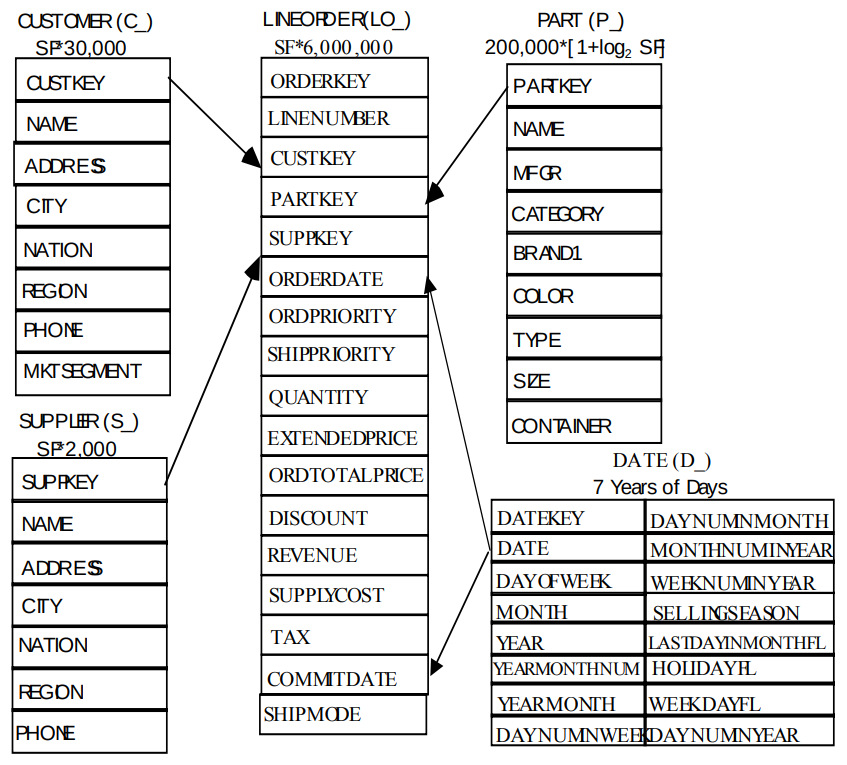
\includegraphics[width=1\textwidth]{pictures/ssb/ssb-schema.png}
    \caption{Schema des \ac{SSB}~\cite{oneil_star_2009}}      % caption the image
    \label{pic:ssb-schema}    % label the image for internal referencing
\end{figure}


\subsubsection{Queries des \ac{SSB}}
Die Queries des \ac{SSB} unterscheiden sich von denen des \ac{TPC-H}.
Der \ac{SSB} nutzt nur Queries, die genau eine SELECT-Anweisung auf der Faktentabelle LINEORDER nutzen und somit keine self-joins nutzen. %self-joins bissl weirder Ausdruck
Die LINEORDER Tabelle wird dann mit einer oder mehreren Dimensionstabellen gejoint und die Ergebnisse somit gefiltert. 
%TODO: Alle SSB SQL-Queries in den Anhang packen

Die Queries des \ac{SSB} sind in vier Kategorien aufgeteilt (query flights): % query flights bissl weird

%TODO: \usepackage{underscore}

\paragraph{Q1}
%ausbauen
Queries in Q1 schränken die Daten über nur eine Dimension, \textbf{DATE}, ein.
Die Faktentabelle \emph{LINEORDER} wird mit der Dimensionstabelle\emph{DATE} gejoint und die Daten anhand einer Zeitspanne aus der DATE-Tabelle und den Bereichen der Felder \emph{lo\_discount} und \emph{lo\_quantity} aus der LINEORDER-Tabelle gefiltert.
Anschließend wird der Umsatz als Summe der Produkte der Felder \emph{lo\_extendedprice} und \emph{lo\_discount} berechnet und als \emph{revenue} zurückgegeben \cite{oneil_star_2009}.


\begin{lstlisting}[
    language=SQL,
    caption=SQL Query-Struktur für Q1 des \ac{SSB},
    label=code:ssb-q1-structur-example
]
SELECT 
    SUM(lo_extendedprice * lo_discount) AS revenue
FROM 
    lineorder, date
WHERE 
    lo_orderdate = d_datekey
    AND d_year = [YEAR]
    -- Specific values below
    AND lo_discount BETWEEN [DISCOUNT] - 1 AND [DISCOUNT] + 1
    AND lo_quantity < [QUANTITY];
\end{lstlisting}

\paragraph{Q2}
In Q2 schränken die Queries die Daten über zwei Dimensionen ein: \textbf{PART} und \textbf{SUPPLIER}.
Anschließend wird wie in Q1 der Umsatz gebildet, wobei die Ergebnisse hier noch nach \emph{d\_year} und \emph{p\_brand1} gruppiert und sortiert werden.  
In Q2 werden insgesamt vier Tabellen (\emph{LINEORDER}, \emph{PART}, \emph{SUPPLIER}, \emph{DATE}) gejoint.
\begin{lstlisting}[
    language=SQL,
    caption=SQL Query-Struktur für Q2 des \ac{SSB},
    label=code:ssb-q2-structur-example
]
SELECT 
    SUM(lo_revenue) AS total_revenue, d_year, p_brand1
FROM 
    lineorder, date, part, supplier
WHERE 
    lo_orderdate = d_datekey
    AND lo_partkey = p_partkey
    AND lo_suppkey = s_suppkey
    AND p_category = 'MFGR#12'
    AND s_region = 'AMERICA'
GROUP BY 
    d_year, p_brand1
ORDER BY 
    d_year, p_brand1;

\end{lstlisting}

\paragraph{Q3}
In Q3 schränken die Queries die Daten über drei Dimensionen ein: \textbf{DATE}, \textbf{SUPPLIER} und \textbf{CUSTOMER}.
Wie in Q1 und Q2 werden auch hier die Umsätze gebildet.
Anschließend werden sie nach \emph{c\_nation}, \emph{s\_region} und \emph{d\_year} gruppiert und nach \emph{d\_year} sortiert.
Es werden insgesamt vier Tabellen (\emph{LINEORDER}, \emph{DATE}, \emph{SUPPLIER} und \emph{CUSTOMER}) gejoint.
\begin{lstlisting}[
    language=SQL,
    caption=SQL Query-Struktur für Q3 des \ac{SSB},
    label=code:ssb-q3-structur-example
]
SELECT 
    c_nation, s_nation, d_year, SUM(lo_revenue) AS revenue
FROM 
    customer, lineorder, supplier, date
WHERE 
    lo_custkey = c_custkey
    AND lo_suppkey = s_suppkey
    AND lo_orderdate = d_datekey
    AND c_region = 'ASIA'
    AND s_region = 'ASIA'
    AND d_year >= 1992
    AND d_year <= 1997
GROUP BY 
    c_nation, s_nation, d_year
ORDER BY 
    d_year ASC, revenue DESC;
\end{lstlisting}

\paragraph{Q4}
Die Queries von Q4 schränken die Daten basierend auf drei Dimensionen (\textbf{CUSTOMER}, \textbf{SUPPLIER} und \textbf{PART}) ein.
Auch hier wird wieder der Umsatz berechnet.
Dieses Mal wird er durch \emph{d\_year} und \emph{c\_nation} gruppiert und sortiert.
Hier werden erstmals alle fünf Tabellen (\emph{LINEORDER}, \emph{CUSTOMER}, \emph{SUPPLIER}, \emph{PART} und \emph{DATE}) gejoint.
\begin{lstlisting}[
    language=SQL,
    caption=SQL Query-Struktur für Q4 des \ac{SSB},
    label=code:ssb-q4-structur-example
]
SELECT 
    d_year, c_nation, SUM(lo_revenue - lo_supplycost) AS profit
FROM 
    date, customer, supplier, part, lineorder
WHERE 
    lo_custkey = c_custkey
    AND lo_suppkey = s_suppkey
    AND lo_partkey = p_partkey
    AND lo_orderdate = d_datekey
    AND c_region = 'AMERICA'
    AND s_region = 'AMERICA'
    AND (p_mfgr = 'MFGR#1' OR p_mfgr = 'MFGR#2')
GROUP BY 
    d_year, c_nation
ORDER BY 
    d_year, c_nation;

\end{lstlisting}
\section{Redis}

Redis ist ein Key-Value Store, der vollständig im Arbeitsspeicher (in-memory) arbeitet und heute häufig als Datenbank, Cache, Message Broker oder Streaming Engine eingesetzt wird~\cite{redis_ltd_introduction_nodate}.
In Redis können unterschiedliche Datenstrukturen verwendet werden. Dazu gehören Strings, Hashes, Listen, Sets, sortierte Sets, Bitmaps, Bitfields, georäumliche Indizes, Streams sowie HyperLogLog~\cite{redis_ltd_data_nodate}.
Mit Erweiterungen, so genannten Modulen, können weitere Datentypen wie z.B. JSON oder Time series unterstützt werden.
Redis wird von vielen bekannten Unternehmen wie GitHub, StackOverflow, Snapchat, Craigslist oder X verwendet~\cite{redis_ltd_whos_nodate}.
Redis wird immer kostengünstiger einsetzbar, da die Arbeitsspeicher im Preis immer weiter fallen~\cite{bergai_trends_2020}.

Des weiteren besteht mit \enquote{Auto Tiering} die Möglichkeit, Arbeitsspeicher zusammen mit SSD-Speicher zu nutzen was die Infrastrukturkosten um bis zu 70\% senken kann~\cite{redis_ltd_auto_nodate}. Dieses Feature ist jedoch nur mit \enquote{Redis Enterprise} möglich.


% Hier ist was doppelt, muss überprüft werden (wahrscheinlich untere lassen, obere entfernen)

Redis ist eine vielseitige Datenbank, die sich nicht streng als herkömmliche Datenbank kategorisieren lässt. Obwohl Redis die grundlegenden Anforderungen an eine traditionelle Datenbank erfüllt, wie das Sammeln und Speichern von Informationen, die dann leicht abgerufen, bearbeitet oder gelöscht werden können, bietet Redis zusätzliche Funktionen, die vor allem durch die Geschwindigkeit aufgrund der vollständigen Ausführung im Arbeitsspeicher und die vielseitigen Datenstrukturen ermöglicht werden.
Durch die Persistierung der Daten auf der Festplatte kann Redis als konventionelle Datenbank genutzt werden.

Außerdem kann Redis als Cache und Message Broker dienen.

Die hohe Geschwindigkeit von Redis erlaubt eine vorteilhafte Verbindung mit anderen Datenbanken, wodurch Redis als optimale Wahl für den Cache von anderen, oft langsameren Datenbanken gilt. So kann Redis beispielsweise genutzt werden um in Echtzeit mit Nutzern zu interagieren währen die Historie der Transaktionen in einer anderen Datenbank gespeichert wird.

Redis bietet als Message-Broker dank des Publish-Subscribe-Paradigmas eine Lösung, um publizierte Nachrichten effizient über bestimmte Kanäle an Abonnenten zu verteilen. Hierbei hat Redis durch seine vielseitigen Datenstrukturen oft Vorteile gegenüber anderen etablierten Message-Brokern~\cite{joshi_you_nodate}.

\subsection{Module für Redis}
\subsubsection{Redis Stack}


\subsection{Datentypen in Redis}
\subsubsection{Strings}
Strings in Redis sind grundlegende Datentypen, die eine Folge von Bytes repräsentieren.
Sie können verschiedene Inhalte wie Text, serialisierte Objekte oder binäre Datenarrays repräsentieren und sind auf eine maximale Größe von 512 MB beschränkt.
Diese Strings unterstützen bitweise Operationen und Funktionen wie Zähler, die durch atomare Inkremente und Dekremente gegen Race-Conditions bei gleichzeitigem Zugriff mehrerer Clients geschützt sind.

Die primären Befehle für die Arbeit mit Strings sind \emph{SET} und \emph{GET}, die das Setzen und Abrufen von Werten ermöglichen, während \emph{MSET} und \emph{MGET} das gleichzeitige Setzen oder Abrufen mehrerer Werte erlauben.

Obwohl die meisten String-Operationen eine konstante Ausführungszeit von O(1) haben und somit sehr effizient sind, benötigen einige Operationen wie \emph{SUBSTR}, \emph{GETRANGE} oder \emph{SETRANGE} eine Ausführungszeit von O(n)~\cite{redis_ltd_strings_nodate}.

\subsubsection{Hashes}
Hashes in Redis dienen als essenzielle Strukturen für die Speicherung von Key-Value-Paaren und ähneln in ihrer Funktionsweise den HashMaps in Java oder Dictionaries in Python. Sie eignen sich insbesondere für die Darstellung grundlegender Objekte und das Speichern von Zählergruppierungen. Ein Hash in Redis kann bis zu \(2^{32} - 1\) Felder enthalten, was eine umfangreiche Kapazität für die Datenorganisation bietet.

In Hashes können beispielsweise Daten von Nutzern einer Applikation wie Vorname, Nachname, Emailadresse gespeichert werden.
Hashes können auch genutzt werden um Daten aus relationalen Datenbanken in Redis darzustellen indem die Spalten als Keys genutzt werden. Jeder Hash stellt so eine Zeile aus einer relationalen Datenbank dar.

Für die Arbeit mit Hashes stellt Redis verschiedene Befehle bereit. Der Befehl \emph{HSET} ermöglicht das Setzen mehrerer Felder eines Hashes, wohingegen \emph{HGET} für das Abrufen des Wertes eines einzelnen Feldes genutzt wird. \emph{HMGET} bietet eine ähnliche Funktion wie \emph{HGET}, gibt jedoch die Werte mehrerer Felder in Form eines Arrays zurück.

Bei der Betrachtung der Performance von Hash-Befehlen in Redis zeichnen sich die meisten durch eine Effizienz mit einer Komplexität von O(1) aus. Allerdings gibt es auch Befehle wie \emph{HKEYS}, \emph{HVALS} und \emph{HGETALL}, deren Komplexität O(n) beträgt, wobei n für die Anzahl der Feld-Wert-Paare im Hash steht. Diese Differenzierung in der Performance ist bei der Anwendung von Hashes in Redis entscheidend, um eine optimale Effizienz und Leistung zu gewährleisten.

~\cite{redis_ltd_hashes_nodate}.
\subsubsection{Listen}
Der Listen-Datentyp in Redis besteht aus verketteten Listen von String-Werten. Er wird häufig verwendet, um Stacks und Queues zu implementieren sowie Queue-Management-Systeme für Hintergrundprozesse zu bauen.
Die maximale Länge einer Redis-Liste beträgt \(2^{32} - 1\) (4.294.967.295) Elemente.

Die grundlegenden Befehle zum Manipulieren von Listen sind \emph{LPUSH} und \emph{RPUSH}, um Elemente am Anfang oder Ende der Liste hinzuzufügen, \emph{LPOP} und \emph{RPOP}, um Elemente von den entsprechenden Enden zu entfernen, und \emph{LLEN}, um die Länge der Liste zu ermitteln.
\emph{LMOVE} und \emph{LTRIM} erlauben das Verschieben von Elementen zwischen Listen oder das Begrenzen von Listen auf eine bestimmte Anzahl von Elementen.

In Redis unterstützen Listen blockierende Befehle wie \emph{BLPOP} und \emph{BLMOVE}, die warten, bis Elemente verfügbar sind, bevor sie Operationen ausführen.
Dies ist besonders nützlich für die Implementierung von Warteschlangen und Prozesskommunikation. So müssen Clients nicht durchgängig neue Anfragen senden falls keine neuen Daten verfügbar sind.
Bibliotheken wie \emph{Resque} und \emph{Sidekiq} nutzen diese Funktionen zur Verwaltung von Hintergrundjobs in Ruby.
Twitter nutzt Redis-Listen zur Speicherung der neuesten Tweets.

Redis-Listen sind effizient beim Hinzufügen sowie Entfernen von Elementen an beiden Enden, da diese Operationen unabhängig von der Listenlänge in konstanter Zeit (O(1)) ausgeführt werden.
Damit eignen sie sich ideal für Echtzeitanwendungen, die schnelle Aktualisierungen erfordern. 
Operationen wie \emph{LINDEX}, die einen Zugriff auf ein Element mitten in der Liste erfordern, sind langsamer, da die benötigte Zeit mit der Position des Elements in der Liste skaliert (O(n)).
Redis-Listen bieten jedoch die Möglichkeit, sie als begrenzte Sammlungen für Anwendungen zu verwenden, bei denen nur die letzten N Einträge von Interesse sind.
In diesem Fall wird die Operation \emph{LTRIM} verwendet, um die Liste auf eine feste Anzahl von Elementen zu beschränken.


Redis erstellt und entfernt Schlüssel automatisch beim Erstellen oder Leeren von Listen~\cite{redis_ltd_lists_nodate}.


\subsubsection{Sets}
Sets in Redis sind eine Datenstruktur für ungeordnete Sammlungen einzigartiger Strings.
Sie eignen sich daher gut für Aufgaben wie das Speichern aller verschiedenen Besucher-IDs einer Webseite oder das Erfassen aller Mitarbeiter einer bestimmten Unternehmensabteilung.
Des Weiteren erlauben Sets die Ausführung gängiger Mengenoperationen wie Schnittmengen, Vereinigungen und Differenzen.
Ein Set kann bis zu \(2^{32} - 1\) Elemente enthalten, was 4.294.967.295 Elementen entspricht.

Die Kernbefehle für die Arbeit mit Sets umfassen \emph{SADD}, um ein neues Element hinzuzufügen, \emph{SREM}, um ein bestimmtes Element zu entfernen, \emph{SISMEMBER}, um die Zugehörigkeit eines Strings zu testen, \emph{SINTER}, um die Schnittmenge von zwei oder mehr Sets zu ermitteln, und \emph{SCARD}, um die Größe eines Sets zu bestimmen.
Zum Entfernen von Elementen aus einem Set kann der Befehl \emph{SREM} verwendet werden, um ein oder mehrere Elemente zu entfernen, oder der Befehl \emph{SPOP}, um ein zufälliges Element zu entfernen.
Der Befehl \emph{SRANDMEMBER} gibt ein zufälliges Element zurück, ohne es zu entfernen.

Neben trivialen gibt es auch komplexe Operationen, die mit den geeigneten Redis-Befehlen einfach zu implementieren sind.
Eine Buchhandlung kann zum Beispiel den \emph{SINTER}-Befehl in Redis verwenden, um Kunden herauszufinden, die in verschiedenen Ländern wie Deutschland und Frankreich ein gemeinsames Interesse an einem Genre, zum Beispiel Science-Fiction, haben.
Zusätzlich zur Schnittmenge können auch Vereinigungs- und Differenzmengen gebildet werden.

Die meisten Operationen wie das Hinzufügen, Entfernen oder Überprüfen der Zugehörigkeit eines Elements zu einem Set sind mit einer Laufzeit von O(1) sehr effizient.
Der Befehl \emph{SMEMBERS} hingegen ist mit O(n) zu bewerten und kann insbesondere bei großen Sets zu langen Ausführungszeiten führen, da er das gesamte Set zurückgibt.
Als Alternative bietet sich der Befehl \emph{SSCAN} an, der ein iteratives Abfragen der Set-Inhalte ermöglicht.

Sets werden oft als Index verwendet. Für eine effiziente Verwaltung von Indizes innerhalb von Redis empfiehlt sich aber das \emph{RediSearch}-Modul~\cite{redis_ltd_sets_nodate}.


\subsubsection{Sortierte Sets (Sorted Sets)}
% \emph Nutzung überprüfen
Ein \emph{Sorted Set} in Redis repräsentiert eine Menge an einzigartigen Strings, die basierend auf einer zugehörigen \emph{Score}-Wertung geordnet sind. Diese Datenstruktur eignet sich besonders für Anwendungsfälle wie Ranglisten oder die Implementierung eines \emph{Rate Limiters} mittels eines gleitenden Zeitfensters (\emph{sliding-window}). Der wesentliche Vorteil eines \emph{Sorted Sets} gegenüber einem herkömmlichen Set liegt in der sofortigen Sortierung der Elemente bei der Einfügung und nicht erst bei der Abfrage. % Limiter überprüfen

Jeder \emph{Score} ist als Gleitkommazahl definiert, wobei die Sortierung primär nach dem \emph{Score} erfolgt. Bei identischen \emph{Scores} bestimmt die lexikographische Reihenfolge der Strings die Positionierung der Elemente. Die Einzigartigkeit der Strings garantiert dabei eine klare Ordnung innerhalb des Sets. Es ist möglich, die \emph{Scores} nachträglich zu aktualisieren, und bei erneutem Einfügen eines Elements wird sowohl der \emph{Score} als auch die Position angepasst, mit einem Rechenaufwand von \(O(\log(N))\), wobei \(N\) die Anzahl der Elemente im Set ist.

Die grundlegenden Befehle für die Arbeit mit \emph{Sorted Sets} sind \emph{ZADD} zum Hinzufügen oder Aktualisieren des \emph{Scores} von Elementen, \emph{ZREM} zum Entfernen von Elementen, \emph{ZRANGE} zum Zurückgeben von Mitgliedern in einem bestimmten Bereich (optional mit \emph{Scores} über `WITHSCORES`), \emph{ZRANGEBYSCORE} zum Abrufen von Elementen in einem bestimmten \emph{Score}-Bereich, und \emph{ZRANK} bzw. \emph{ZREVRANK} zur Ermittlung des Rangs eines Elements in aufsteigender oder absteigender Sortierreihenfolge.

Für lexikographische Bereiche stehen Befehle wie \emph{ZRANGEBYLEX}, \emph{ZREVRANGEBYLEX}, \emph{ZREMRANGEBYLEX} und \emph{ZLEXCOUNT} zur Verfügung.

Die meisten Operationen auf \emph{Sorted Sets} haben eine Laufzeit von \(O(\log(n))\), mit Ausnahme von \emph{ZRANGE}, dessen Laufzeit \(O(\log(n) + m)\) beträgt, wobei \(m\) die Anzahl der zurückzugebenden Elemente ist.

Technisch gesehen sind \emph{Sorted Sets} durch eine duale Datenstruktur realisiert, die eine Skip-List und eine Hash-Tabelle kombiniert, sodass jede Einfügung eine \(O(\log(N))\) Operation darstellt. Die vorsortierte Natur der \emph{Sorted Sets} ermöglicht einen effizienten Zugriff ohne zusätzlichen Sortieraufwand bei der Abfrage.

Obwohl \emph{Sorted Sets} auch für die Indizierung verwendet werden können, ist für den Aufbau eines effizienten Index in Redis das Modul RediSearch zu empfehlen~\cite{redis_ltd_sorted-sets_nodate}.


\subsubsection{Streams}
Redis Streams sind eine Datenstruktur in Redis, die als anhängbares Protokoll (append-only log) fungiert und gleichzeitig mehrere Operationen zur Überwindung der Grenzen typischer anhängbarer Protokolle implementiert. Diese umfassen unter anderem den wahlfreien Zugriff (\enquote{random access}) in O(1)-Zeit und komplexe Konsumstrategien wie Verbrauchergruppen.
Die Anwendungsbereiche von Redis Streams sind vielfältig und schließen Event Sourcing, Sensorüberwachung und Benachrichtigungssysteme ein.

Falls nicht anders vorgegeben generiert Redis für jeden Eintrag in einem Stream automatisch eine eindeutige ID, die auch Zeitinformationen beinhaltet, was den effizienten Abruf und Bereichsabfragen ermöglicht.

Grundlegende Befehle zur Interaktion mit Redis Streams sind \emph{XADD} für das Hinzufügen, \emph{XREAD} für das Lesen, \emph{XRANGE} für Bereichsabfragen und \emph{XLEN} zur Bestimmung der Länge eines Streams.

Consumer Groups in Redis sorgen für eine effiziente Verteilung von Nachrichten, indem sie sicherstellen, dass jede Nachricht nur einmal an einen Konsumenten geliefert wird. Dies ermöglicht auch die Nachverfolgung von noch nicht bestätigten Nachrichten. Zur Überwachung und Verwaltung dieser Streams und Consumer Groups dienen Befehle wie \emph{XPENDING} und \emph{XINFO}.

Die Begrenzung der Datenspeicherung in Redis Streams wird durch den \emph{MAXLEN}-Parameter im \emph{XADD}-Befehl realisiert.

Wie andere Redis-Datenstrukturen werden Streams asynchron auf Repliken repliziert und in AOF- sowie RDB-Dateien persistiert, einschließlich der Zustände von Consumer Groups.

Das Hinzufügen eines Eintrags zu einem Redis Stream ist eine O(1)-Operation, während der Zugriff auf einzelne Einträge als O(n)-Operation charakterisiert wird, wobei n die Länge der ID darstellt. In der Regel sind diese IDs kurz, was zu einem relativ konstanten Zeitaufwand führt, allerdings kann dieser Aufwand variieren, je nach spezifischer Anwendung und Struktur der IDs~\cite{redis_ltd_streams_nodate}.

\subsubsection{Bitmaps}
Bitmaps sind in Redis kein eigener Datentyp sondern eine Reihe an bit-orientierten Operationen auf dem String-Datentyp der wie ein Bit-Vektor genutzt wird. Da Strings in Redis binärsicher sind und eine maximale Länge von 512 MB aufweisen, eignen sie sich gut, um bis zu \(2^{32}\) unterschiedliche Bits zu setzen.
Bitweise Operationen lassen sich sowohl auf einzelne als auch auf mehrere dieser Strings anwenden.

Bitmaps können so für eine effiziente Darstellung von Sets, bei denen die Mitglieder des Sets den ganzen Zahlen von 0 bis N entsprechen, genutzt werden.

Ein praktisches Anwendungsbeispiel für Bitmaps in Redis ist ein Parkhaus-Verwaltungssystem, in dem jeder Parkplatz durch ein Bit repräsentiert wird. Hierbei werden belegte Parkplätze durch ein Bit im Wert 1 und freie Parkplätze durch ein Bit im Wert 0 dargestellt.

Redis bietet einige grundlegende Befehle zur Arbeit mit Bitmaps. Der Befehl \emph{SETBIT} dient dazu, ein Bit an einem bestimmten Offset auf 0 oder 1 zu setzen, während \emph{GETBIT} den Wert eines Bits an einem gegebenen Offset zurückgibt. Mit \emph{BITOP} lassen sich bitweise Operationen an einem oder mehreren Strings durchführen. \emph{BITCOUNT} führt eine Populationszählung durch und berichtet die Anzahl der auf 1 gesetzten Bits. \emph{BITPOS} schließlich findet das erste Bit mit dem spezifizierten Wert von 0 oder 1.

Es gibt zwei Kategorien von Bitoperationen: die konstantzeitigen Einzelbit-Operationen, wie das Setzen oder Abrufen eines Bitwertes, und Operationen auf Bitgruppen, wie das Zählen der Anzahl gesetzter Bits in einem bestimmten Bereich. Diese zweite Kategorie umfasst beispielsweise die Populationszählung.

Bitmaps bieten den großen Vorteil, dass sie häufig erhebliche Speicherplatzersparnisse bei der Speicherung von Informationen ermöglichen.Zum Beispiel kann in einem System, das Benutzer über fortlaufende IDs identifiziert, ein Bit pro Benutzer genutzt werden, um eine einfache Information wie den Wunsch, einen Newsletter zu erhalten, zu speichern. Mit dieser Methode lassen sich solche Daten für bis zu 4 Milliarden Benutzer mit nur 512 MB Speicher verwalten.

Die Performance von Bitmap-Befehlen in Redis variiert je nach Art der Operation. Die Befehle \emph{SETBIT} und \emph{GETBIT} werden in konstanter Zeit, also in O(1), ausgeführt. Der Befehl \emph{BITOP} hat hingegen eine Ausführungszeit von O(n), wobei n die Länge des längsten Strings in der Vergleichsoperation darstellt~\cite{redis_ltd_bitmaps_nodate}.


\subsubsection{Bitfields}
Wie Bitmaps, so werden auch Bitfelder (\emph{\enquote{Bitfields}}) in Redis in Zeichenketten gespeichert. Diese sind jedoch binär kodiert. Bitfelder in Redis ermöglichen es, Ganzzahlen beliebiger Bitlänge zu setzen, zu inkrementieren und abzufragen. Man kann beispielsweise mit Ganzzahlen arbeiten, die von vorzeichenlosen 1-Bit-Integers bis zu vorzeichenbehafteten 63-Bit-Integers reichen.

Bitfelder unterstützen atomare Lese-, Schreib- und Inkrementierungsoperationen, was sie zu einer guten Wahl für die Verwaltung von Zählern und ähnlichen numerischen Werten macht. So können Bitfelder beispielsweise verwendet werden, um einfache Statistiken in einem Videospiel zu führen, wie etwa die Anzahl einer bestimmten Währung, wie Diamanten, oder die Anzahl der Tode.

Die Anzahl der Diamanten könnte beispielsweise am Offset 0 und die Anzahl der Tode am Offset 1 gespeichert werden. Die Breite dieser Zähler könnte auf 32 Bit festgelegt werden.

Der Befehl \emph{BITFIELD} in Redis ermöglicht das atomare Setzen, Inkrementieren und Lesen von Werten, während \emph{BITFIELD\_RO} als schreibgeschützte Variante dient, die speziell für leseintensive Anwendungen optimiert ist.


Die Leistung des Befehls \emph{BITFIELD} ist O(n), wobei n die Anzahl der zugegriffenen Zähler darstellt~\cite{redis_ltd_bitfields_nodate}.


\subsubsection{Geodatenindizes}
Der Datentyp \enquote{\textbf{Geospatial}} ermöglicht die Speicherung und Abfrage von Koordinaten in Redis. So können z.B. nahegelegene Punkte innerhalb eines bestimmten Radius oder eines definierten Begrenzungsrahmens ermittelt werden.
Ein praktisches Anwendungsbeispiel für diese Funktionalität wäre eine mobile Anwendung, die dem Benutzer die nächstgelegenen Elektroroller in seiner Umgebung anzeigt.

Zwei grundlegende Befehle sind in diesem Zusammenhang von zentraler Bedeutung: Der Befehl \emph{GEOADD} fügt einen Standort zu einem gegebenen georäumlichen Index hinzu, wobei zu beachten ist, dass bei diesem Befehl der Längengrad vor dem Breitengrad angegeben wird. Der Befehl \emph{GEOSEARCH} hingegen gibt Standorte innerhalb eines bestimmten Radius oder einer bestimmten Begrenzung zurück~\cite{redis_ltd_geospatial_nodate}.





\subsubsection{HyperLogLog}
\ac{HLL} ist eine probabilistische Datenstruktur in Redis, die Schätzung der Kardinalität einer Menge ermöglicht und dabei bis zu 12 KB Speicher verwendet. Diese Implementierung zeichnet sich durch einen Standardfehler von 0,81\% aus und kann Mengen mit bis zu \(2^{64}\) Mitgliedern schätzen.

Im Gegensatz zur traditionellen Zählung einzigartiger Elemente, die einen Speicherplatz proportional zur Elementanzahl erfordert, bietet \ac{HLL} eine Speicherplatz-effiziente Schätzung mit einem geringen Fehleranteil.

Technisch gesehen unterscheidet sich \ac{HLL} von anderen Datenstrukturen in Redis, wird jedoch als Redis-String kodiert, wodurch \emph{GET} zur Serialisierung und \emph{SET} zur Deserialisierung eines \ac{HLL} genutzt werden kann.

Konzeptionell ähnelt die Nutzung von \ac{HLL} in einigen Aspekten dem Einsatz von Sets, insbesondere in der Verwaltung einzigartiger Elemente. Die direkte Speicherung der Elemente erfolgt jedoch nicht, stattdessen wird ein Zustand aufgezeichnet, der für Schätzungen verwendet wird.

Anwendungsbereiche von \ac{HLL} umfassen beispielsweise die Zählung einzigartiger Suchanfragen oder die Bestimmung der Anzahl einzigartiger Besucher einer Webseite.

Bei den grundlegenden Befehlen für die Arbeit mit \ac{HLL} in Redis, erlaubt \emph{PFADD} das Eintragen eines Elements in ein \ac{HLL}. Die Anzahl der Elemente in einem \ac{HLL} lässt sich mit \emph{PFCOUNT} schätzen. Für das Zusammenführen von mehreren HyperLogLogs steht der Befehl \emph{PFMERGE} zur Verfügung.

Hinsichtlich der Leistungsfähigkeit zeichnen sich Schreib- (\emph{PFADD}) und Leseoperationen (\emph{PFCOUNT}) bei HyperLogLogs durch konstante Zeit- und Speicheranforderungen aus. Das Konsolidieren mehrerer HyperLogLogs mittels \emph{PFMERGE} stellt eine O(n)-Operation dar, wobei n die Anzahl der zu vereinenden HLLs repräsentiert.
~\cite{redis_ltd_hyperloglog_nodate}.


\subsubsection{Weitere Datentypen durch zusätzliche Module}
Durch Module können in Redis zusätzliche Datentypen wie zum Beispiel \emph{JSON} oder \emph{Time-Series}-Daten genutzt werden.

Das \textbf{RedisJSON}-Modul bietet eine Unterstützung für JSON-Daten in Redis.
JSON-Daten können so direkt in der Redis-Datenbank gespeichert, aktualisiert und wieder abgerufen werden, was eine effiziente Verwaltung von komplexen Datenstrukturen ermöglicht. Hierzu zählen das gezielte Bearbeiten von Subelementen dank der \emph{JSONPath}-Syntax und ein schneller Zugriff auf Unterstrukturen von JSON-Dokumenten.
Außerdem ermöglicht RedisJSON atomare Operationen auf Datentypen innerhalb der JSON-Dokumente, um die Leistungsfähigkeit bei der Datenaufbereitung zu verbessern.
Ein wesentlicher Vorteil im Vergleich zur Speicherung von JSON als serialisierte Strings besteht in der Fähigkeit, JSON-Objekte zu indizieren und zu durchsuchen, was im Zusammenspiel mit dem \emph{RediSearch}-Modul ermöglicht wird.
Dadurch können komplexe Anfragen direkt in Redis ausgeführt werden~\cite{redis_ltd_json_nodate, redis_json-use-cases_nodate}.

Durch das \textbf{RedisTimeSeries}-Modul können Zeitreihendaten in Redis gespeichert werden.
Dabei bietet Redis hohe Einfügeraten und schnelle Lesezugriffe.
Es ermöglicht Abfragen innerhalb spezifizierter Start- und Endzeiten sowie eine Vielfalt von aggregierten Abfragen, einschließlich, aber nicht beschränkt auf Minimum, Maximum, Durchschnitt und Summe, für beliebige Zeitintervalle.
Zudem lässt sich ein maximaler Aufbewahrungszeitraum konfigurieren und die Kompaktierung sorgt für automatisch aktualisierte, aggregierte Zeitreihen.
Durch die Verwendung von sekundären Indizes, welche auf Labels (Feld-Wert-Paare) basieren, können Zeitreiheneinträge gezielt abgefragt werden.
Die Daten können außerdem in anderen metrischen Programmen, wie beispielsweise Prometheus oder Grafana, weitergenutzt werden~\cite{redis_ltd_time_nodate}.


% Eventuell Abschnitt umstrukturieren

\subsection{Redis Cluster}
% https://learning.oreilly.com/library/view/mastering-redis/9781783988181/ch06.html#ch06lvl1sec42
% https://learning.oreilly.com/library/view/redis-4-x-cookbook/9781783988167/d590a8d8-2532-4601-9568-a52ccdcbec6f.xhtml

\section{RediSearch}

RediSearch ist ein Redis-Modul, das es ermöglicht, nach Daten in Redis über Indizes zu suchen.
Es unterstützt die Durchsuchung von HASH- und JSON-Werten, wobei letzteres das zusätzliche Modul \emph{RedisJSON} voraussetzt.
RediSearch verfügt über eine eigene Abfragesprache, die es auch ermöglicht, komplexere Suchanfragen und Aggregationen durchzuführen~\cite{redis_ltd_search_nodate}. %Wo Zitat hin?

RediSearch bietet verschiedene Such- und Abfragefunktionen.
So können Abfragen über mehrere Felder hinweg durchgeführt werden.
Zudem bietet es Aggregationsfunktionen und volltextbasierte Indexierung mehrerer Felder in einem Dokument.
Eine inkrementelle Indexierung ist ohne Leistungseinbußen möglich, sodass ein Index zuerst erstellt und danach eigenständig von Redis verwaltet sowie an sich ändernde Daten angepasst werden kann.

Weitere Funktionen umfassen logische Abfragen mithilfe von Operatoren wie \emph{AND}, \emph{OR} und \emph{NOT}, optionale Filterklauseln, präfixbasierte Suchen, Feldgewichtungen, Autovervollständigung und vage Präfix-Vorschläge (\enquote{Fuzzy-Prefix-Vorschläge}).
Es werden exakte Phrasensuchen und Distanzabhängige Suchen (\enquote{slop-basiert}) unterstützt. Darüber hinaus gibt es \emph{Stemming}-basierte Abfrageerweiterungen für viele Sprachen, einschließlich Deutsch und Englisch, mittels \emph{Snowball}.
RediSearch bietet eine begrenzte Unterstützung für benutzerdefinierte Funktionen zur Erweiterung und Bewertung von Suchanfragen (\enquote{Scoring}).

Zusätzlich dazu umfasst RediSearch numerische Filter und Bereichsabfragen, Geo-Filterung unter Verwendung von Redis-Geo-Befehlen und Suchfunktionen für Vektoren, die für semantische Suchaufgaben sowohl exakte als auch approximative Algorithmen verwenden.
Es unterstützt Unicode und ermöglicht das Abrufen von vollständigen Dokumentinhalten oder nur deren IDs.

RediSearch kann auch in verteilten Datenbank-Clustern eingesetzt werden.
\subsection{Interner Aufbau von RediSearch}
\subsubsection{Redis String DMA} % Ist das noch relevant?
\emph{Redis String DMA} ermöglicht es Redis-Modulen, Daten auf \enquote{Redis-String-Schlüssel} zu mappen. Sie erhalten dann direkte Zeiger auf die Daten, ohne diese kopieren oder serialisieren zu müssen.
Durch die Verwendung von \enquote{Redis String DMA} zum Kodieren von invertierten Indizes ermöglicht RediSearch einen schnellen Zugriff auf große Speichermengen~\cite{redis_ltd_internal_nodate}.


\subsubsection{Indizes in RediSearch}
Die derzeit verfügbare Dokumentation auf \emph{redis.io}~\cite{redis_ltd_internal_nodate} ist zum Zeitpunkt dieser Arbeit nicht mehr aktuell und bezieht sich auf Versionen vor der Einführung von RediSearch 2.0.
Mit der Einführung von Version 2.0 wurden erhebliche Änderungen vorgenommen, die von den in der Dokumentation beschriebenen Funktionalitäten wesentlich abweichen.
Diese Änderungen werden am Ende dieses Kapitels behandelt.
Es ist jedoch zu beachten, dass die nachfolgenden Informationen hauptsächlich auf der veralteten Dokumentation beruhen.

RediSearch implementiert invertierte Indizes innerhalb von Redis.
Es verwendet eine angepasste Datenkodierung (\enquote{\emph{Redis String DMA}}), die eine effiziente Speicher- und CPU-Suche ermöglicht.

Früher wurden solche Indizes als Sets direkt in Redis gespeichert, was speicherintensiv war und keine Kodierung von Offsets erlaubte. Seit Version 2.0 von RediSearch werden die Daten der Indizes separat gespeichert.

\subsubsection{Invertierte Indizes}
Der Invertierte Index in RediSearch enthält für jedes indizierte Wort bzw. Suchparameter eine Liste an Dokumenten, in denen es vorkommt.
Zusätzlich werden weitere Daten gespeichert, wie etwa die Häufigkeit und die Stellen, an denen der Suchbegriff im Dokument auftritt (\enquote{Offset}).
Bei einer Suche kann entweder ein einzelner Index oder eine Verbindung mehrerer Indizes nach dem Suchbegriff durchsucht werden.

Zusätzlich zu den invertieren Indizes werden weitere Daten in anderen \textit{Redis DMA string keys} gespeichert:\\
Der sogenannte \textbf{Skip-Index}, eine Tabelle des Index-Offsets von einem Fünfzigstel der Einträge im Index. Dies ermöglicht eine schnellere Suche, wenn mehrere invertierte Indizes überschnitten werden, da nicht die gesamte Liste durchsucht werden muss.\\
Da bei der Suche nach einzelnen Wörtern nicht alle Treffer durchsucht werden, sondern nur die ersten N Treffer für den Benutzenden relevant sind, wird für jeden Suchbegriff ein Hilfsindex mit den ersten 20 oder mehr Einträgen erstellt, der sogenannte \textbf{Score Index}.

Beim indizieren konnte früher angegeben werden, dass die Inhalte der Dokumente nicht gespeichert werden. Diese Option ist jedoch seit Version 2.0 von RediSearch nicht mehr verfügbar~\cite{redis_ltd_upgrade_nodate, korland_missing_nodate}.
% Hier eigentlich "Document and result ranking" aber veraltet ?!
% Sollte hier mehr ins Detail gegangen werden, was genau gespeichert wird?

\subsection{Nutzung von RediSearch} % Das müsste nen Überkapitel sein...

\subsection{Grundstrukturen in RediSearch}
Die Grundelemente von RediSearch sind in der Online-Dokumentation von Redis beschrieben~\cite{redis_ltd_basic_nodate}.
Sie bestehen aus \emph{Documents}, \emph{Fields} und dem \emph{Schema}.

\emph{Documents} sind die Basiseinheiten der Information, eindeutig identifizierbar durch ihren Schlüsselnamen, bestehend aus \emph{Hash}- oder \emph{JSON}-Datenobjekten. Jedes \emph{Document} enthält mehrere \emph{Fields}, die spezifische Attribute oder Eigenschaften repräsentieren und unterschiedliche Datentypen enthalten können. Bei einem Hash sind dies die einzelnen Elemente innerhalb des Hash und bei JSON die Felder des Dokuments.
Das \emph{Schema} definiert die Struktur des Index. Es legt fest, wie die \emph{Fields} gespeichert und indiziert werden.

Für eine effiziente Suche ist es wichtig, nur relevante \emph{Fields} zu indizieren, da die Indizierung aller \emph{Fields} zu unnötigem Overhead führen kann. Nicht indizierte \emph{Fields} tragen nicht zu den Suchergebnissen bei, können aber als Teil der \emph{Document}-Daten beim Abrufen der Suchergebnisse abgerufen werden. Aggregationen (siehe [VERWEIS AUF SPÄTERE KAPITEL]) können nur mit indizierten Feldern arbeiten. % TODO: Verweis auf Aggregation

\subsection{Anlegen von Inidizes}
Indizes werden in RediSearch mithilfe des Befehls \emph{FT.CREATE} erstellt.
Die Verwendung des Befehls wird in der Online-Dokumentation~\cite{redis_ltd_ftcreate_nodate} von Redis erläutert.
Die Syntax für die Erstellung lautet wie folgt:
\begin{lstlisting}[
    language=TEXT,
    caption=Syntax des Befehls FT.CREATE in RediSearch,
    label=code:redisearch-ftcreate-syntax,
    numbers=none
]
FT.CREATE index 
  [ON HASH | JSON] 
  [PREFIX count prefix [prefix ...]] 
  [FILTER {filter}]
  [LANGUAGE default_lang] 
  [LANGUAGE_FIELD lang_attribute] 
  [SCORE default_score] 
  [SCORE_FIELD score_attribute] 
  [PAYLOAD_FIELD payload_attribute] 
  [MAXTEXTFIELDS] 
  [TEMPORARY seconds] 
  [NOOFFSETS] 
  [NOHL] 
  [NOFIELDS] 
  [NOFREQS] 
  [STOPWORDS count [stopword ...]] 
  [SKIPINITIALSCAN]
  SCHEMA field_name [AS alias] TEXT | TAG | NUMERIC | GEO | VECTOR | GEOSHAPE [ SORTABLE [UNF]] 
  [NOINDEX] [ field_name [AS alias] TEXT | TAG | NUMERIC | GEO | VECTOR | GEOSHAPE [ SORTABLE [UNF]] [NOINDEX] ...]
\end{lstlisting}

Die Erstellung eines Indexes in RedisSearch mittels des Befehls \emph{FT.CREATE} beinhaltet eine Reihe von Konfigurationsoptionen, die es ermöglichen, den Index an spezifische Anforderungen anzupassen.
Dabei sind nur die Argumente \emph{index} und \emph{SCHEMA} verpflichtend anzugeben. Alle anderen Argumente sind optional und werden im folgenden nur kurz erläutert.

Das Argument \emph{index} dient zur Angabe des Namens des zu erstellenden Indexes.

Innerhalb des \emph{SCHEMA}-Teils des Befehls werden die zu indizierenden Felder definiert. Der \emph{\{identifier\}} legt das Feld im Hash oder den JSON-Pfad-Ausdruck fest, während \emph{AS \{attribute\}} es erlaubt, einem Identifikator einen Aliasnamen zuzuweisen. Die verschiedenen Feldtypen und Optionen des Schemas werden in \ref{sec:redisearch-schema-fieldtypes} erläutert.


Das Argument \emph{ON \{data\_type\}} bestimmt die Datentypen, auf die der Index angewendet wird. Standardmäßig wird HASH verwendet, während JSON als alternative Option existiert.

Über \emph{PREFIX \{count\} \{prefix\}} werden die vom Index zu erfassenden Schlüssel bestimmt. Mehrere Präfixe können hinzugefügt werden, standardmäßig werden alle Schlüssel indiziert.

Der Ausdruck \emph{FILTER \{filter\}} erlaubt die Nutzung der RediSearch-Aggregationssprache für spezifische Filterungen.

Durch \emph{LANGUAGE \{default\_lang\}} und \emph{LANGUAGE\_FIELD \{lang\_attribute\}} werden die Standardsprache und das Sprachattribut des Dokuments festgelegt.

\emph{SCORE \{default\_score\}} und \emph{SCORE\_FIELD \{score\_attribute\}} definieren den Standardwert für die Dokumentenbewertung und das Attribut für die Benutzerrangfolge.

\emph{PAYLOAD\_FIELD \{payload\_attribute\}} ermöglicht es, ein Dokument mit einer binär sicheren Nutzlastzeichenfolge zu versehen.

Das Argument \emph{MAXTEXTFIELDS} zwingt RediSearch dazu, Indizes so zu kodieren, als ob sie mehr als 32 Textattribute enthalten, um die Flexibilität bei der Erweiterung zu erhöhen.

\emph{NOOFFSETS} verzichtet auf die Speicherung von Termoffsets, was Speicherplatz spart, aber gewisse Suchfunktionen einschränkt.

\emph{TEMPORARY \{seconds\}} erstellt einen temporären Index, der nach einer vorgegebenen Zeitspanne verfällt.

\emph{NOHL} deaktiviert die Hervorhebungsfunktion, um Speicherplatz zu sparen, während \emph{NOFIELDS} und \emph{NOFREQS} die Speicherung von Attributbits bzw. Häufigkeiten von Begriffen im Index unterbinden.

Mit \emph{STOPWORDS \{count\}} kann eine benutzerdefinierte Stoppwortliste festgelegt werden, und \emph{SKIPINITIALSCAN} vermeidet das sofortige Scannen und Indizieren von Dokumenten.




\subsection{Feldtypen und Optionen des Schemas}\label{sec:redisearch-schema-fieldtypes}
RediSearch bietet eine Auswahl an Feldtypen (\emph{field types}) für verschiedene Indexierungszwecke. Folgend werden die verschiedenen Feldtypen erläutert. Die Informationen stammen dabei, falls nicht anders angegeben, aus der Online-Dokumentation von Redis zu Feldtypen~\cite{redis_ltd_field_nodate} und dem \emph{FT.CREATE}-Befehl~\cite{redis_ltd_ftcreate_nodate}.

\subsubsection{\emph{Number fields}}
Nummernfelder speichern zählbare Werte in Ganzzahl- oder Gleitkommazahlen und erlauben sortierbare Bereichsabfragen. Sie können mit dem \emph{FT.CREATE}-Befehl wie folgt definiert werden:\\
\texttt{FT.CREATE ... SCHEMA ... {field\_name} NUMBER [SORTABLE] [NOINDEX]}

Bedeutung der Optionen \emph{SORTABLE} und \emph{NOINDEX}:

- \emph{SORTABLE}: Ermöglicht die Sortierung des Feldes, nützlich für Bereichsabfragen und Sortierung von Suchergebnissen.

- \emph{NOINDEX}: Das Feld wird nicht indiziert, nützlich für Texte, die abrufbar, aber nicht durchsuchbar sein sollen.

Ein Beispiel für eine Query mit einem numerischen Filter könnte wie folgt sein:\\
\texttt{FT.SEARCH recipeIndex "@cooking\_time:[10 30]"}

Queries unterstützen außerdem Syntax die angibt ob der Bereich vollständig einschließend, vollständig ausschließend , mit einer offenen Ober- oder Untergrenze sein soll. Zusätzlich kann auch explizit nach einem bestimmten Wert gesucht werden in dem die Grenzen des Bereichs die gleiche Zahl sind. Außerdem kann eine Filterbedingung auch negiert werden.

\subsubsection{\emph{Geo fields}} Diese Felder sind für geografische Koordinaten vorgesehen, die Radiusabfragen für standortbezogene Suchfunktionen ermöglichen.
Sie können mit dem \emph{FT.CREATE}-Befehl wie folgt definiert werden:\\
\texttt{FT.CREATE ... SCHEMA ... \{field\_name\} GEO [SORTABLE] [NOINDEX]}

Die Optionen \emph{SORTABLE} und \emph{NOINDEX} entsprechen denselben Optionen wie bei \emph{numeric fields}. 

Der Syntax zur Abfrage von Geo-Feldern sieht wie folgt aus:\\
\texttt{@<field\_name>:[<lon> <lat> <radius> <unit>]}

Um etwa Orte im Umkreis von 100 Kilometern um die Position von Furtwangen zu finden kann folgender Befehl genutzt werden:\\
\texttt{FT.SEARCH cities "@coords:[8.20 48.05 100 km]"}

% TODO: Checken ob der Abschnitt so gut ist.
\subsubsection{\emph{Geoshape fields}}
Geosphape-Felder sind die neuesten Feldoptionen in RediSearch. Sie sind noch nicht in allen Dokumentationen vermerkt. Die Informationen beziehen sich auf die Dokumentation des \emph{FT.CREATE}-Befehls~\cite{redis_ltd_ftcreate_nodate} und die Dokumentation über Queries~\cite{redis_ltd_query_nodate}. 
Geoshapes ermöglichen geografische Abfragen mit der WKT-Notationen (\enquote{well-known text}).
Es werden sowohl Punkte wie auch Polygone unterstützt. Sie werden in einem Text wie folgt definiert:\\
\texttt{POINT(2 4)} oder \texttt{POLYGON((2 2, 2 8, 6 11, 10 8, 10 2, 2 2))}

Ein Eintrag kann dann beispielsweise so erstellt werden:\\
\texttt{HSET shape:1 t "this is my house" g "POLYGON((2 2, 2 8, 6 11, 10 8, 10 2, 2 2))"}


Mit den Optionen \emph{FLAT} oder \emph{SPHERICAL} kann angegeben werden, ob die Koordinaten kartesisch  oder  geografisch sind.

Der Syntax für Queries zur Abfrage lautet wie folgt:\\
\texttt{@field:[{WITHIN|CONTAINS} \$geometry] PARAMS 2 geometry \{geometry\}}

Ein Beispiel, in dem abgefragt wird, ob ein Polygon einen bestimmten Punkt beinhaltet könnte so aussehen:\\
\texttt{FT.SEARCH polygon\_idx "@g:[CONTAINS \$point]" PARAMS 2 point 'POINT(8 8)' DIALECT 3
}
\emph{DIALECT 3} gibt bei mehrwertigen Attributen statt Skalaren JSON zurück.
Komplexere Beispiele und Erklärungen sind in der Dokumentation zu Queries~\cite{redis_ltd_query_nodate} zu finden.


\subsubsection{\emph{Vector fields}} Vektor-Felder halten Gleitkommavektoren, die diverse unstrukturierte Daten wie etwa Text oder Bilder repräsentieren können, und unterstützen Vektorsimilaritätssuchen. Sie werden oft für externe Machine-Learning-Modelle genutzt.

Die Felder können mit dem \emph{FT.CREATE}-Befehl definiert werden:\\
\texttt{FT.CREATE ... SCHEMA ... {field\_name} VECTOR {algorithm} {count} [{attribute\_name} {attribute\_value} ...]
}

Mit dem \emph{algorithm}-Attribut wird ein unterstützter Algorithmus für Vektorvergleiche angegeben. Er wird genutzt bei der Suche nach den k ähnlichsten Vektoren im Index oder beim Filtern von Vektoren nach Bereichen. Die unterstützten Algorithmen sind \emph{FLAT} für einen \enquote{brut force} Algorithmus und \emph{HNSM} für einen \enquote{hierarchical, navigable, small world} Algorithmus.

Das \emph{count}-Attribut gibt an, wie viele Attributpaare im Befehl verwendet werden. Wobei die Attributpaare die Algorithmusattribute für die Erstellung des Vektorindexes sind. Jeder Algorithmus hat seine eigenen obligatorischen und optionalen Attribute.

Ein Index kann zum Beispiel so erstellt werden:\\
\texttt{FT.CREATE my\_idx SCHEMA vec\_field VECTOR FLAT 6 TYPE FLOAT32 DIM 128 DISTANCE\_METRIC L2}

Ein Beispiel für einen Vektorvergleich ist der \enquote{k nearest neighbors}(KNN)-Algorithmus. Die Syntax dazu ist wie folgt aufgebaut:\\
\texttt{*=>[ KNN {num|\$num} @vector \$query\_vec ]}\\
Eine Abfrage nach den zehn nächsten Nachbarn bei denen \enquote{query\_vec} am nächsten zum Vektor der in \enquote{@vector\_field} gespeichert ist sieht so aus:\\
\enquote{*=>[KNN 10 @vector\_field \$query\_vec]}

Weitere Informationen und komplexere Beispiele sind in den Dokumentationen zu Queries~\cite{redis_ltd_query_nodate} und zu Vektoren~\cite{redis_ltd_vectors_nodate} zu finden.


\subsubsection{\emph{Tag fields}} In Tag-Feldern werden Textdaten als Tags oder Labels gespeichert, die ohne Tokenisierung verarbeitet werden. Sie eignen sich gut zur Datenorganisation und -kategorisierung.

Tags werden beim Erstellen des Index mit dem \emph{FT.CREATE}-Befehl wie folgt erstellt:\\
\texttt{FT.CREATE ... SCHEMA ... {field\_name} TAG [SEPARATOR {sep}] [CASESENSITIVE]}

Der \emph{SEPARATOR} kann zur Angabe des Zeichens verwendet werden, das zum Trennen mehrerer Tags in einem Feld verwendet werden soll (Standard ist ein Komma).

\emph{CASESENSITIVE} gibt an, ob bei Tags die Groß- und Kleinschreibung zu beachten ist. Standardmäßig wird bei Tag-Feldern nicht zwischen Groß- und Kleinschreibung unterschieden (\enquote{\emph{caseinsensitive}}).

Um nach Tags zu suchen wird folgende Syntax verwendet:\\
\texttt{@<field\_name>:\{<tag>\}}\\
Um etwa nach Rezepten mit Tomaten als Zutat zu suchen, kann folgender Befehl verwendet werden:\\
\texttt{FT.SEARCH recipeIndex "@ingredients:\{tomato\}"}


\subsubsection{{\emph{Text fields}}}
Textfelder sind für die Speicherung menschlicher Sprache optimiert. Sie werden zu Kleinbuchstaben umgewandelt und tokenisiert, um effiziente Volltextsuchen zu ermöglichen. Zudem können sie gewichtet und sortiert werden, was eine differenzierte Suchrelevanz und -ordnung ermöglicht.
Textfelder können mit dem FT.CREATE Befehl wie folgt angegeben werden:\\
% Hier vllt. nen fancigen codeblock aber ohne untertitel und so
\texttt{FT.CREATE ... SCHEMA ... \{field\_name\} TEXT [WEIGHT] [NOSTEM] [PHONETIC \{matcher\}] [SORTABLE] [NOINDEX] [WITHSUFFIXTRIE]}

Die Bedeutung der einzelnen Optionen:

- \emph{WEIGHT}: Gewichtet das Feld, um bestimmten Feldern bei der Suche mehr Bedeutung zu geben.

- \emph{NOSTEM}: Verhindert das Stemming des Feldes, nützlich für nicht zu tokenisierende Texte wie URLs.

- \emph{PHONETIC \{matcher\}}: Führt eine phonetische Übereinstimmung durch. Es können verschiedene \emph{matcher} für verschiedene Sprachen angegeben werden.

- \emph{WITHSUFFIXTRIE}: Indiziert das Feld mit einem Suffix-Trie, optimiert für Contains- und Suffix-Anfragen.

- Die Optionen \emph{SORTABLE} und \emph{NOINDEX} haben den gleichen Effekt wie bei \emph{Number fields}.

Die Suche nach Dokumenten mit bestimmten Textwerten ist möglich durch die Verwendung von \emph{<term>} oder \emph{@<field\_name>}:
\{<term>\} in der Abfragesyntax. Zum Beispiel:

% TODO: LatexProblem fixen, falsche Anführungszeichen (muss "" sein)
- Suche in allen Textattributen: \texttt{FT.SEARCH recipeIndex \glqq egg\grqq}

- Suche nur im Preparation-attribut: \texttt{FT.SEARCH recipeIndex "@preparation:boil"}




% TODO: Dieses Kapitel ergibt eventuell mehr Sinn vor dem vorherigen, da sich manche Beispiele auf diesen Index beziehen
\subsection{Anlegen eines Beispielindexes}
Das Indexschema legt die Felder, deren Typen sowie die Indizierungs- und Speicherregeln fest und ist entscheidend für die Effizienz der Suchfunktionalität sowie der Speichernutzung.
Die Definition des Schemas erfolgt bei der Indexerstellung mit dem Befehl \emph{FT.CREATE}~\cite{redis_ltd_ftcreate_nodate}.
Im Folgenden wird die Erstellung eines Index anhand eines Beispiels erläutert.
Der Index soll für das Rezeptverzeichnis eines Kochbuches verwendet werden.

\begin{lstlisting}[
    language=TEXT,
    caption=Beispiel eines Befehls zum Anlegen eines Index in RediSearch,
    label=code:redisearch-creation-of-index-example
]
FT.CREATE recipeIndex
    ON HASH
    PREFIX 1 recipe:item:
SCHEMA
    name TEXT WEIGHT 5.0
    preparation TEXT
    ingredients TAG
    category TAG
    difficulty TAG
    cooking_time NUMERIC SORTABLE
\end{lstlisting}

Das Attribut\emph{ON HASH} gibt an, dass Hash-Dokumente indexiert werden sollen. Alternativ kann hier noch \emph{ON JSON} für JSON-Dokumente verwendet werden.
Der Prefix legt fest, dass nur Dokumente, die mit der angegebenen Zeichenfolge beginnen, indexiert werden. Zusätzlich zu diesen Attributen gibt es noch weitere optionale Attribute die in der Dokumentation des \emph{FT.CREATE}-Befehls erläutert werden, auf die hier jedoch nicht weiter eingegangen wird.
In diesem Fall initiiert der Befehl die Erstellung eines Index mit dem Namen \emph{recipeIndex}, der auf Hash-Dokumente mit dem Schlüsselanfang \emph{recipe:item:} angewendet wird. 
Das Schema dieses Index enthält die Felder \emph{name}, \emph{preparation}, \emph{ingredients}, \emph{category}, \emph{difficulty} und \emph{cooking\_time}.

Der Datentyp \emph{TEXT} wird für \emph{name} und \emph{preparation} verwendet, um die Textinformationen der Rezeptnamen und Zubereitungsanweisungen zu indizieren. Die Verwendung des Typs \emph{TAG} für \emph{ingredients} und \emph{category} erleichtert die Handhabung kategorisierter Daten wie Zutatenlisten und Rezeptkategorien. \emph{cooking\_time}, klassifiziert als \emph{NUMERIC} und \emph{SORTABLE}, ermöglicht die Suche und Sortierung nach Kochzeit. Das Feld \emph{difficulty} dient zur Angabe des Schwierigkeitsgrades des Rezeptes.

Dem Feld \emph{name} wird ein Gewicht von 5.0 zugewiesen, um seine Relevanz bei Suchanfragen zu erhöhen. Dieser Index ermöglicht eine effiziente Suche im Rezeptverzeichnis und das Filtern der Ergebnisse nach Kriterien wie Zutaten, Kategorie, Kochzeit und Schwierigkeitsgrad.

\subsection{Aggregations}
Aggregationen (Aggregations) stellen die effektivste Methode dar, um in Redis mit RediSearch Daten abzufragen. Die hier dargestellten Informationen basieren auf den Erklärungen, die in der Online-Dokumentation~\cite{redis_ltd_aggregations_nodate} von Redis zu finden sind.

Aggregationen ermöglichen die Verarbeitung und Analyse von Suchergebnissen durch verschiedene Operationen wie Gruppierung, Sortierung und Daten-Transformation. Ähnlich wie bei anderen Datenbanken sollen diese Verfahren dazu beitragen, analytische Erkenntnisse aus den Daten zu gewinnen. Des Weiteren können mit Aggregationen facettierte Suchanfragen durchgeführt werden. Suchergebnisse können so anhand verschiedener Merkmale oder \enquote{Facetten} gefiltert und verfeinert werden.

Ein Beispiel für den Einsatz einer Aggregation in RediSearch wäre eine OLAP-Abfrage, die berechnet wie oft Rezepte die Tomaten enthalten in den letzten drei Monaten aufgerufen wurden.

\subsubsection{Aufbau einer Aggregation}
Eine Aggregation-Query ist in zwei Teile unterteilt:\\
Zu Beginn wird eine Suche durchgeführt, bei der relevante Datensätze ausgewählt und gefiltert werden.
Anschließend wird eine Verarbeitungspipeline aufgebaut, bei der die Datensätze nach bestimmten Feldern gruppiert, sortiert, transformiert, limitiert und oder gefiltert werden. Die verschiedenen Schritte in einer Verarbeitungspipeline können beliebig oft ausgeführt werden und haben folgende Effekte:

- \emph{Group and reduce}: Gruppierung von Datensätzen nach bestimmten Feldern und Anwendung von Reduktionsfunktionen auf jede Gruppe, um aggregierte Daten zu erhalten.
    
- \emph{Sort}: Sortierung von Ergebnissen basierend auf einem oder mehreren Feldern.
    
- \emph{Apply transformations}: Anwenden von mathematischen Funktionen und Zeichenkettenfunktionen auf Felder in der Pipeline, wobei optional neue Felder erstellt oder bestehende Felder ersetzt werden können.
    
- \emph{Limit}: Begrenzung der Ergebnismenge, unabhängig von der Sortierreihenfolge, um eine handhabbare Datenmenge zu gewährleisten.
    
- \emph{Filter}: Nachträgliche Filterung der Ergebnisse auf der Grundlage von Prädikaten, die sich auf die Werte der Datensätze beziehen, um die Daten weiter zu verfeinern.

\subsubsection{Syntax einer Aggregation}
Aggregationen werden mit dem Befehl \emph{FT.AGGREGATE} ausgeführt der folgende Syntax hat:
\begin{lstlisting}[
    language=TEXT,
    caption=Syntax des Befehls FT.AGGREGATE in RediSearch,
    label=code:redisearch-ftaggregate-syntax,
    numbers=none
]
FT.AGGREGATE
  {index_name:string}
  {query_string:string}
  [VERBATIM]
  [LOAD {nargs:integer} {property:string} ...]
  [GROUPBY
    {nargs:integer} {property:string} ...
    REDUCE
      {FUNC:string}
      {nargs:integer} {arg:string} ...
      [AS {name:string}]
    ...
  ] ...
  [SORTBY
    {nargs:integer} {string} ...
    [MAX {num:integer}] ...
  ] ...
  [APPLY
    {EXPR:string}
    AS {name:string}
  ] ...
  [FILTER {EXPR:string}] ...
  [LIMIT {offset:integer} {num:integer} ] ...
  [PARAMS {nargs} {name} {value} ... ]
\end{lstlisting}

Bei Parametern, die eine variable Anzahl an Argumenten haben, ist das erste Argument immer die Anzahl der Argumente {nargs:integer}. So werden Mehrdeutigkeiten beim Parsen zu vermieden, wenn eines der Argumente den gleichen Namen wie ein anderer Parameter hat.

Nachfolgend werden die einzelnen Argumente und ihre Parameter erläutert:

\emph{index\_name}: Der Name des zu verwendenden Index.

\emph{query\_string}: Die Basisabfrage. Sie folgt der Syntax der Suchabfrage, inklusive Filter und Operatoren.

\emph{LOAD \{nargs\} \{property\} ...}: Lädt Dokumentfelder aus Hash-Objekten, beeinträchtigt jedoch die Leistung, Felder sollten wenn möglich als SORTABLE gespeichert werden. Es ist jedoch notwendig Felder zu laden, die nicht SORTABLE sind, um sie in weiteren Schritten der Pipeline zu nutzen.

\emph{GROUPBY \{nargs\} \{property\} ...}: Gruppiert Ergebnisse nach einer oder mehrerer Eigenschaften. Jede Gruppe sollte zusätzlich einen \emph{Reducer} haben (siehe nächsten Punkt).

\emph{REDUCE \{func\} \{nargs\} \{arg\} ... [AS \{name\}]}: Reduziert Ergebnisse jeder Gruppe zu einem einzelnen Eintrag mittels einer Reduktionsfunktion wie etwa \emph{COUNT.} Optional kann das so entstandene Feld mit \enquote{AS \{name\}.} benannt werden, andernfalls wird ein Name generiert der sich aus der Reduktionsfunktion und den Gruppeneigenschaften zusammensetzt.

\emph{SORTBY \{nargs\} \{property\} \{ASC|DESC\} [MAX \{num\}]}: Sortiert Ergebnisse nach Eigenschaften. Standardmäßig aufsteigend, umkehrbar mit ASC oder DESC. Mit dem Attribut \emph{MAX} kann die Sortierung optimiert werden in dem sie nur die n-größten Elemente sortiert.

\emph{APPLY {expr} AS {name}}: Führt eine Transformation auf Eigenschaften aus. \emph{expr} beinhaltet Berechnungen oder Funktionen auf numerischen oder anderen Eigenschaftstypen. Das Ergebnis wird als neue Eigenschaft mit \emph{AS {name}} gespeichert und ist in nachfolgenden Operationen verwendbar.

\emph{LIMIT \{offset\} \{num\}}: Begrenzt die Anzahl der Ergebnisse die zurückgegeben werden. Dabei wird die Anzahl der Ergebnisse festgelegt und ab welchem Offset sie ausgewählt werden sollen. Falls die Ergebnisse auch sortiert werden ist es effizienter, sie mit dem Attribut \emph{MAX} des Befehls \emph{SORTBY} zu limitieren.

\emph{FILTER \{expr\}}: Filtert Ergebnisse mit Prädikatausdrücken, bezogen auf aktuelle Pipelinewerte.

\emph{PARAMS \{nargs\} \{name\} \{value\}}: Definiert Parameter für die Abfrage die aus einem Namen und einem Wert bestehen. Parameter können in der Abfrage durch \$-Zeichen und dem Namen referenziert werden. Jede Referenz in der Suchanfrage auf einen Parameternamen wird dann durch den entsprechenden Parameterwert ersetzt.

\section{Scala} % Todo: Eventuell ausbauen
Scala ist eine moderne Programmiersprache die Merkmale objektorientierter und funktionaler Sprachen aufweist.
Sie zeichnet sich außerdem durch eine starke Typisierung aus.
Ihre Syntax zeigt Parallelen zu Java auf, und es ist möglich, Java-Funktionen sowie Java-Libraries in Scala zu verwenden~\cite{epfl_scala_nodate-1, epfl_introduction_nodate}.
Scala läuft in der JVM, mit JavaScript im Browser oder nativ mit LLVM~\cite{epfl_scala_nodate}.

\subsection{Einsatzgebiete von Scala}
Auf dem \emph{\acf{PYPL}} belegt Scala im November 2023 den 20. Platz der beliebtesten Programmiersprachen~\cite{carbonnelle_pypl_2023}.
Durch die Kompatibilität mit Java eigenet sich Scala auch für alle gängigen Einsatzgebiete von Java. 
Durch Scalas besondere Eigenschaften eignet es sich jedoch besonders für hochdurchsatzfähige HTTP-Server und -Clients, in Form von Skripten für die Kommandozeile, mit JavaScript im Frontend-Web sowie für die Datenverarbeitung.

Scala wird außerdem häufig mit \emph{Akka}~\cite{lightbend_akka_nodate} für verteilte Anwendungen verwendet.

\subsection{Vorteile von Scala}
Scala hat einige Charakteristiken, die ihm im Vergleich zu Java einen Vorteil verschaffen.
Besonders zu betonen sind folgende Eigenschaften von Scala im Gegensatz zu Java~\cite{epfl_scala_nodate-1, epfl_scala_nodate-2}: % Quellenangabe hier so okay?

\begin{enumerate}
    \item \textbf{Kompakterer und ausdrucksstärkerer Code:} Scala ermöglicht oftmals kürzere und prägnantere Codezeilen im Vergleich zu Java. Dies wird durch spezifische Konstrukte in Scala, wie \emph{case}-Klassen und Collections-Operationen (\emph{map} und \texttt{toMap}), sowie durch Pattern Matching erreicht, was den Code weniger umfangreich und einfacher lesbar macht.
    
    \item \textbf{Funktionale Programmierung:} Scala, eine Sprache, die objektorientierte und funktionale Programmierstile unterstützt, bietet Vorteile durch funktionale Konzepte wie Higher-Order-Funktionen und effiziente Methoden zur Transformation von Collections. Diese Eigenschaften sind in Java oft weniger elegant umsetzbar oder erfordern mehr Boilerplate-Code.
    
    \item \textbf{Immutability und Case Classes:} Der Einsatz von Unveränderlichkeit (Immutability) bei der Definition von Datenstrukturen ist in Scala weniger komplex als in Java. Scala's \emph{case}-Klassen unterstützen Unveränderlichkeit und Pattern Matching, was die Sicherheit und Wartbarkeit des Codes erhöht.
    
    \item \textbf{Pattern Matching:} Scalas Implementierung von Pattern Matching ermöglicht eine elegantere und sicherere Handhabung potenziell fehlender Werte, ein Ansatz, der in Java nicht so nativ und leserlich umgesetzt ist.
    
    \item \textbf{Typinferenz:} Durch Scala's Typinferenz wird der Bedarf an expliziten Typdeklarationen reduziert, was den Code weniger überladen und besser lesbar macht – ein Aspekt, der in Java oft durch die Notwendigkeit expliziter Typangaben nicht gegeben ist.
\end{enumerate}


\subsection{Redis mit Scala (Jedis)} %subsection oder subsubsection?
Jedis ist ein Java-Client für Redis, der sich durch hohe Leistung und einfache Benutzbarkeit auszeichnet. Als Hauptvorteile bietet Jedis fortgeschrittene Unterstützung für verschiedene Redis-Versionen, eine effiziente Handhabung potenziell fehlender Werte durch Pattern Matching sowie eine Unterstützung für Redis-Module wie RediSearch~\cite{redis_inc_jedis_2023}.
Da Scala mit Java-Bibliotheken kompatibel ist lässt sich Jedis mit wenig Mehraufwand auch in Scala nutzen. % -> Hier Verweis auf Implementierungskapitel wo kurz erklärt wird dass man die scla-java-converter nutzen muss.

Grundsätzlich gibt es Bibliotheken für die Arbeit mit Redis in vielen Programmiersprachen und der Quellcode, der während dieser Arbeit erstellt wurde, wäre auch in anderen modernen Programmiersprachen wie etwa Java oder Python möglich gewesen.
Die Entscheidung für Scala in dieser Arbeit basiert auf den oben genannten Vorteilen und der persönlichen Präferenz des Autors.


\section{Lua}
Lua ist eine Programmiersprache, die auf ihrer offiziellen Webseite als mächtige, effiziente, leichtgewichtige und integrierbare Skriptsprache beschrieben wird~\cite{ierusalimschy_lua_nodate}. Die Sprache unterstützt eine Vielzahl von Programmierparadigmen wie prozedurale Programmierung, objektorientierte Programmierung, funktionale Programmierung, datengesteuerte Programmierung und Datenbeschreibung. Die Informationen in den folgenden Abschnitten stammen, sofern nicht anders angegeben, von der offiziellen Lua-Webseite.

\subsection{Einsatzgebiete von Lua}
Auf dem \emph{\acf{PYPL}} belegt Lua im November 2023 den 21. Platz der beliebtesten Programmiersprachen~\cite{carbonnelle_pypl_2023}.

Aufgrund ihrer geringen Größe wird Lua häufig als Skriptsprache innerhalb von Anwendungen verwendet. Ein Beispiel hierfür ist \emph{Fusion 18}~\cite{blackmagic_design_fusion_nodate}, eine in Hollywood häufig verwendete Compositing-Software. Auch in der Videospielbranche wird Lua häufig für Erweiterungen verwendet, z.B. bei \emph{World of Warcraft}~\cite{wowpedia_lua_2023}.

Lua-Skripte können auch innerhalb von \emph{Redis} ausgeführt werden~\cite{redis_ltd_scripting_nodate}. Die Skripte laufen direkt auf dem Redis-Server, was die Interaktion mit Redis sehr effizient macht.
Lua ist kompatibel mit allen Unix- und Windows-Systemen, läuft auf eingebetteten Mikroprozessoren sowie auf Smartphones mit iOS und Android.

Die Programmiersprache verfügt über eine einfache und gut dokumentierte API, die eine enge Integration mit in anderen Sprachen geschriebenem Code ermöglicht. Es ist einfach, Lua mit Bibliotheken zu erweitern, die in anderen Sprachen geschrieben wurden. Ebenso ist es einfach, Programme, die in anderen Sprachen geschrieben wurden, mit Lua zu erweitern.
\subsection{Technische Aspekte}
Die technischen Aspekte werden im \emph{Reference Manual}~\cite{ierusalimschy_lua_nodate-1} erklärt.

Lua wurde als Bibliothek in \emph{clean C} implementiert. Es ist eine dynamisch typisierte Programmiersprache, die Bytecode durch Interpretation mit einer registrierbasierten virtuellen Maschine verarbeitet.

Lua umfasst nur acht grundlegende Datentypen: \emph{nil}, \emph{boolean}, \emph{number}, \emph{string}, \emph{function}, \emph{userdata}, \emph{thread} und \emph{table}.

Der Datentyp \emph{nil} hat ausschließlich den Zweck, sich von allen anderen Datentypen zu unterscheiden und ähnelt dem Datentyp \emph{null} in Java. Der Datentyp \emph{number} repräsentiert sowohl ganze Zahlen als auch reelle Zahlen und wird in die Untertypen \emph{integer} und \emph{float} unterteilt.

Der Datentyp \emph{string} stellt unveränderliche Bytefolgen dar und kann jeden 8-Bit-Wert enthalten. Der Datentyp \emph{thread} steht zur Implementierung von \emph{Coroutinen} unabhängiger Ausführungsstränge bereit und steht nicht im Zusammenhang mit Betriebssystem-Threads.
Lua-Funktionen sowie C-Funktionen werden mit dem Datentyp \emph{function} dargestellt.
Der Datentyp \emph{userdata} dient dazu, C-Daten in Lua-Variablen zu speichern.

In dieser Arbeit findet der Datentyp \emph{table} besondere Beachtung, der assoziative Arrays implementiert, die nicht nur Zahlen, sondern auch beliebige Lua-Werte außer \emph{nil} und \emph{NaN} (ein spezieller Wert nach dem IEEE 754 Standard der undefinierte numerische Ergebnisse wie etwa \enquote{0/0} darstellt) als Indizes haben können.
Tabellen sind in Lua der einzige Mechanismus zur Strukturierung von Daten. Sie können verwendet werden, um gewöhnliche Arrays, Listen, Symboltabellen, Sets, Records, Graphen, Bäume und andere Datentypen darzustellen.

\subsection{Lua in Redis}
Redis ermöglicht das direkte Ausführen von Lua-Skripten auf dem Server, wodurch die Redis-Befehle der Skripte effizient verarbeitet werden können, da diese nicht über das Netzwerk übertragen werden müssen. Diese Skripte garantieren eine atomare Ausführung, bei welcher sämtliche Serveraktivitäten während der Laufzeit des Skripts blockiert sind. Die Möglichkeiten von Lua-Skripten in Redis werden in der Online-Dokumentation von Redis erläutert~\cite{redis_ltd_scripting_nodate}.

Durch die Möglichkeit eigene Funktionen für komplexe Aufrufe zu erstellen, wird Redis mittels Skripten leicht erweiterbar. Die meisten \emph{Redis-Befehle} können in \emph{Lua-Skripten} genutzt werden.

Unterschieden werden muss bei der Verwendung von Lua-Skripten in Redis zwischen klassischen Skripten, die mit dem \emph{EVAL}-Befehl ausgeführt werden, und den sogenannten \emph{Redis Functions}~\cite{redis_ltd_redis_nodate-1}. Klassische Skripte erfordern bei jedem Aufruf durch den \emph{EVAL}-Befehl das Senden des Skripts an den Redis-Server, was zu einem Netzwerk- und Kompilierungs-Overhead führt, wenn Skripte mehrfach verwendet werden sollen.

Im Gegensatz dazu bieten \emph{Redis Functions} dieselbe Funktionalität wie klassische Skripte, aber mit dem Vorteil, dass Redis sie als Teil der Datenbank verwaltet und für ihre Verfügbarkeit sorgt.  So werden \emph{Functions} auch auf der Festplatte persistiert. Sie müssen nur einmalig an den Redis-Server gesendet werden und können dann beliebig oft aufgerufen werden. \Die \emph{Functions} werden als so genannte \emph{Library} verwaltet, wobei eine Library mehrere \emph{Functions} enthalten kann, die sich somit auch Code teilen können.

In der Online-Dokumentation von Redis wird auch die Redis-Lua-API~\cite{redis_ltd_redis_nodate} sowie das Debuggen von Lua-Skripten~\cite{redis_ltd_debugging_nodate} erläutert.


\chapter{SSB in Redis}
% TODO: Kapitel linken
Der \emph{Star Schema Benchmark} wurde ursprünglich für relationale Datenbanken entwickelt, die auf SQL basieren. Er ist nicht ohne weiteres auf Key-Value-Stores wie \emph{Redis} übertragbar. In diesem Kapitel wird erläutert, wie die Daten und Abfragen des SSB angepasst werden können, um den Benchmark in Redis durchführen zu können.

In Kapitel ~\ref{sec:ssb-data-in-redis} werden Ansätze vorgestellt, wie die Daten innerhalb von Redis strukturiert werden können. Im Anschluss daran wird das im Rahmen dieser Arbeit entwickelte Programm \emph{SSB Inserter} zum Einfügen der Daten in Redis vorgestellt.


Kapitel ~\ref{sec:ssb-use-in-redis} beschäftigt sich mit der Ausführung des SSB in Redis.
Zunächst wird das entwickelte Programm \emph{Redis OLAP Client} vorgestellt, welches zur Ausführung der Queries verwendet wurde. Anschließend werden verschiedene Ansätze zur Durchführung der Queries erläutert.

\section{Herausforderungen}
%\subsection{Keine Joins}

% TODO: Irgendwo noch Test von SSB in PostgreSQL
\section{SSB Daten in Redis}\label{sec:ssb-data-in-redis}

% TODO: Hier ganze Anleitung im Anhang verlinken
\subsection{Generieren von SSB Daten}
Um Daten für einen \emph{Star Schema Benchmark} zu generieren, stellen die Autoren ein spezielles Tool~\cite{phillips_electrumssb-dbgen_2023} zur Verfügung.
Das in \emph{C} programmierte Tool ermöglicht nach der Kompilierung die Erstellung von \emph{.tbl}-Dateien, welche für den Import in SQL-basierte Datenbanksysteme geeignet sind.
Es erlaubt die Variation der Datenmenge durch Anpassung eines Parameters, um unterschiedliche Skalierungen zu generieren.
Das Tool basiert auf einem Programm, das ursprünglich zur Datengenerierung für den TPC-H-Benchmark entwickelt wurde.
\begin{lstlisting}[
    caption=Auszug aus generierter supplier.tbl-Datei,
    label=code:ssb-dbgen-example,
    numbers=none
]
92|Supplier#000000092|n48Wy4QI3lm|BRAZIL   7|BRAZIL|AMERICA|12-446-416-8471|
93|Supplier#000000093|wd1djjKXT|MOZAMBIQU9|MOZAMBIQUE|AFRICA|26-359-388-5266|
\end{lstlisting}
Die Zeilen der .tbl-Datei repräsentieren eine Zeile in einer Datenbanktabelle. Die einzelnen Spalten sind durch einen Trennstrich voneinander getrennt.
Beim Importieren der Daten werden die Spalten den entsprechenden Spalten in der Datenbank zugeordnet. Dafür muss die Tabelle im korrekten Format erstellt werden.

\subsection{Sternschema in Redis abbilden}
Bei der Betrachtung der Datenorganisation gibt es grundlegende Unterschiede zwischen dem \emph{Sternschema} und den Möglichkeiten zur Datenmodellierung in \emph{Redis}. Während das Sternschema trotz einer geringeren Normalisierung als einige andere Schemata mehrere Tabellen umfasst, fehlt das Konzept der Tabelle in \emph{Redis} vollständig.

\subsubsection{Modellierung der Daten mit künstlichen Namensräumen}
Um dennoch eine Art Tabellenstruktur in \emph{Redis} zu erreichen, werden durch das Hinzufügen von Präfixen zu Schlüsseln künstliche Namensräume geschaffen. Alle Einträge, die der Tabelle \emph{Supplier} angehören, beginnen beispielsweise mit dem Präfix \enquote{supplier:}. Durch dieses Vorgehen ist es möglich, bei der Nutzung von Befehlen wie \emph{Scan} oder bei der Anwendung von Indizes in \emph{RediSearch} gezielt nach diesem Präfix zu suchen. Die Methode wird dabei von \emph{RedisInsight} unterstützt, das die Möglichkeit bietet, Daten in der Benutzeroberfläche nach Präfixen gruppiert anzuzeigen.

Es besteht die Möglichkeit, mehrere \emph{Datenbanken} in Redis anzulegen.
Dies wird jedoch als Anti-Pattern angesehen und ist daher nicht empfohlen~\cite{prickett_answer_2022}. Viele Erweiterungen unterstützen nur die erste Datenbank. Daher wird der Ansatz der künstlichen Namensräume bevorzugt. 

Neben der Option, die Struktur der \emph{SSB}-Daten durch künstliche Namensräume darzustellen, besteht auch die Möglichkeit, die Daten vollständig zu denormalisieren. Kapitel \ref{sec:ssb-inserter} beschreibt die Umsetzung beider Ansätze.


\subsubsection{Wahl des Datentypen in Redis}
Von den gängigen Datentypen in Redis unterstützen nur Hashes, JSON und Sorted Sets eine Key-Value-Struktur. Theoretisch können Daten auch in Strings gespeichert werden und durch die Volltextsuche von Redisearch ist es auch möglich nach Daten zu suchen, jedoch ist dies wesentlich komplizierter als bei Hashes und JSON.
In Sorted Sets können nur begrenzte numerische Werte gespeichert werden was sie für die SSB-Daten nicht nutzbar macht, da dort unter anderem auch Texte gespeichert werden müssen.
Hashes und JSON bieten beide die Möglichkeit, beliebige Daten in einer Key-Value-Struktur zu speichern und dann mir RediSearch auch nach diesen Daten zu suchen.
Hashes benötigen dafür jedoch erheblich weniger Speicherplatz als JSON.
JSON wird in einer deserialisierten Form gespeichert und benötigt etwas Overhead zusätzlich zu den eigentlichen Daten~\cite{redis_ltd_json-ram-usage_nodate}.
Hashes sind dagegen optimiert um Speicher zu sparen~\cite{redis_ltd_memory-optimization_nodate}.
Mit dem Befehl \texttt{MEMORY USAGE} kann der Speicherverbrauch eines Elements in Redis angezeigt werden~\cite{redis_ltd_memory-usage-command-redis_nodate}.

% Dafür sorgen dass Abbildung an richitger Stelle ist...
In \Cref{pic:redis-hash-vs-json-memory} wird der Vergleich der Speicherplatznutzung dargestellt, wobei dieselben Informationen einmal in Form eines Hash und einmal in Form von JSON gespeichert sind. In diesem Beispiel belegt das JSON-Format 694 Byte, während das Hash-Format nur 288 Byte benötigt, was einer Reduzierung um 58,5\% entspricht.
\begin{figure}[!h]  % force the figure to be placed here
    \centering
    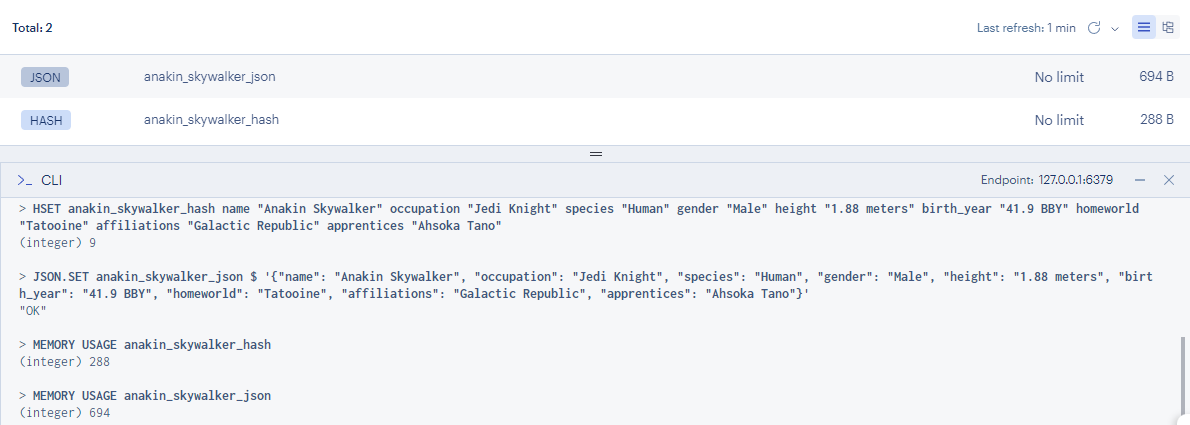
\includegraphics[width=1\textwidth]{pictures/redis/redis_hash_vs_json_memory.png}
    \caption{Vergleich des Speicherplatznutzung zwischen HASH und JSON}
    \label{pic:redis-hash-vs-json-memory}
\end{figure}

\subsection{SSB Inserter}\label{sec:ssb-inserter}

\subsubsection{Konfiguration von RediSearch und Jedis}
Redis verfügt über Eigenschaften, die beim Einfügen großer Datenmengen suboptimal sein können.
Es bietet die Möglichkeit, Daten sowohl als Snapshot als auch in einer Append-Only-Datei zu speichern (siehe Dokumentation von Redis~\cite{redis_ltd_persistence_nodate}).
Beim Einfügen von vielen Daten besteht die Gefahr, dass mehrfach Daten gespeichert werden, die in kurzer Zeit nicht mehr aktuell sind, wenn weitere Daten eingefügt werden. Aus diesem Grund wird beim Start des Programms sichergestellt, dass beide Optionen in der Konfiguration deaktiviert sind. Nachdem die Daten eingefügt wurden werden die Optionen wieder angepasst. 

Jedis hat außerdem einen Timeout für Anfragen. Um sicherzustellen, dass dieser Timeout das Einfügen der Daten nicht beendet, wird er auf unendlich gesetzt.

\begin{lstlisting}[
    caption=Optimierung beim Einfügen von Daten,
    label=code:ssb-inserter-redis-config,
    language=Scala
]
// before inserting
jedis.configSet("appendonly", "no")
jedis.configSet("save", "")
jedis.getClient.setTimeoutInfinite()

// after inserting
jedis.configSet("appendonly", "yes")
jedis.configSet("save", "3600 1")
// perform snapshot every hour if at least one key has been changed
\end{lstlisting}


\subsubsection{Einfügen der Daten mit künstlichen Namensräumen}
% TODO: bissl drumrum ausbauen...
Um die Daten des \emph{SSB} in \emph{Redis} zu integrieren, ist es notwendig, zunächst die generierten \emph{.tbl}-Dateien zu lesen. Da in diesen Dateien keine Informationen zu den Spaltennamen enthalten sind, muss das Programm diese vergeben. Die benötigten Spaltennamen wurden aus dem SQL-Import-Skript entnommen, welches normalerweise zur Erstellung der Tabellen in \emph{PostgreSQL} verwendet wird.

Die Namen der Spalten sind in einem \emph{String}-Array innerhalb des \emph{Scala}-Programms gespeichert, wie in \Cref{code:ssb-inserter-datastructures} dargestellt:

\begin{lstlisting}[
    caption=Arrays mit den Namen der Spalten der SSB-Tabellen,
    label=code:ssb-inserter-datastructures,
    language=Scala
]
val customerStructure: Array[String] =
  Array("c_custkey", "c_name", "c_address", "c_city", "c_nation", "c_region", "c_phone", "c_mktsegment")
val partStructure: Array[String] =
  Array("p_partkey", "p_name", "p_mfgr", "p_category", "p_brand1", "p_color", "p_type", "p_size", "p_container")
val dateStructure: Array[String] =
  Array("d_datekey", "d_date", "d_dayofweek", "d_month", "d_year", "d_yearmonthnum", "d_yearmonth", "d_daynuminweek", "d_daynuminmonth", "d_daynuminyear", "d_monthnuminyear", "d_weeknuminyear", "d_sellingseason", "d_lastdayinweekfl", "d_lastdayinmonthfl", "d_holidayfl", "d_weekdayfl")
val supplierStructure: Array[String] =
  Array("s_suppkey", "s_name", "s_address", "s_city", "s_nation", "s_region", "s_phone")
val lineorderStructure: Array[String] =
  Array("lo_orderkey", "lo_linenumber", "lo_custkey", "lo_partkey", "lo_suppkey", "lo_orderdate", "lo_orderpriority", "lo_shippriority", "lo_quantity", "lo_extendedprice", "lo_ordtotalprice", "lo_discount", "lo_revenue", "lo_supplycost", "lo_tax", "lo_commitdate", "lo_shipmod")

\end{lstlisting}


Der SSB Inserter liest zuerst jede \emph{.tbl}-Datei mit der Methode \texttt{readLines} ein. Dabei wird der Tabellenname aus dem Dateinamen extrahiert und die Datei in Zeilen gelesen. Die gelesenen Zeilen werden in Gruppen zu je 1000 Stück gebündelt. Für jede Gruppe wird die Funktion \texttt{insertIntoRedis} aufgerufen, die die Daten in die Redis-Datenbank einfügt. Dabei wird der Tabellenname, ein Array mit den Spaltennamen, ein Jedis-Pipeline-Objekt und ein Boolean übergeben, der angibt, ob der Tabellenname \emph{lineorder} ist.
Zusätzlich wird die Zeit gemessen, die zum lesen und Einfügen der Daten benötigt wird.

\begin{lstlisting}[
    caption=Die Funktion readLines des SSB Inserter,
    label=code:ssb-inserter-readlines,
    language=Scala
]
def readLines(fileName: String, dataStructure: Array[String], pipeline: Pipeline): Unit = {
	val tableName: String = fileName.split("\\.")(0);
	val startTime = System.nanoTime
	Try(Source.fromFile(fileName)) match {
		case Success(file) =>
			file.getLines().grouped(1000).foreach(s => insertIntoRedis(s, tableName, dataStructure, tableName == "lineorder", pipeline))
			println("Inserted data into " + tableName + " in " + (System.nanoTime() - startTime) + " nanoseconds")
			file.close()
		case Failure(exception) =>
			println("Could not read file `" + fileName + "`. It should be placed into the same folder as the .jar")
			println(exception.getMessage)
	}
}
\end{lstlisting}

Die Funktion \texttt{insertIntoRedis} arbeitet wie folgt: Zunächst werden die vorliegenden Daten, die aus einer Folge von Zeilen bestehen, verarbeitet. Jede Zeile wird dabei anhand des Trennzeichen (\enquote{|}) in einzelne Werte aufgeteilt. Anschließend wird für jedes Schlüsselelement im Array \emph{dataStructure} ein entsprechender Wert aus der aufgeteilten Zeile ausgewählt. Dann wird geprüft, ob die Option \emph{isLineOrder} aktiviert ist. Falls zutreffend, wird der Schlüssel für die Redis-Datenbank aus dem Namen der Datenbank und den ersten beiden Werten der Zeile gebildet. Andernfalls wird der Schlüssel lediglich aus dem Datenbanknamen und dem ersten Wert der Zeile erzeugt. Jedes Schlüssel-Wert-Paar wird dann in der Redis-Pipeline mit einem \emph{hset}-Befehl erzeugt, um den Wert unter dem jeweiligen Schlüssel in der Datenbank zu speichern.

\begin{lstlisting}[
    caption=Die Funktion insertIntoRedis des SSB Inserter,
    label=code:ssb-inserter-insertIntoRedis,
    language=Scala
]
def insertIntoRedis(data: Seq[String], databaseName: String, dataStructure: Array[String], isLineOrder: Boolean, pipeline: Pipeline): Unit = {
	data.foreach(line => {
		val values = line.split("\\|")
		val valueIterator = values.iterator
		dataStructure.foreach(key => {
			if (valueIterator.hasNext) {
				if (isLineOrder) {
					pipeline.hset((databaseName + ":" + values(0) + ":" + values(1)).getBytes, key.getBytes, valueIterator.next().getBytes())
				} else {
					pipeline.hset((databaseName + ":" + values(0)).getBytes, key.getBytes, valueIterator.next().getBytes)
				}
			}
		})
	})
	pipeline.sync()
}
\end{lstlisting}

Um eindeutige Schlüsselnamen zu generieren, wird der Wert, der normalerweise als Primärschlüssel in relationalen Datenbanken verwendet wird, dem Tabellennamen angehängt. In der \emph{lineorder}-Tabelle ist dies ein zusammengesetzter Schlüssel, der aus zwei Feldern besteht. Aus diesem Grund ist es im Code notwendig, zwischen der \emph{lineorder}-Tabelle und den anderen Tabellen zu unterscheiden.

Die Daten werden gebündelt und in einer Pipeline an Redis übermittelt. Durch diese Bündelung auf maximal 1000 Elemente pro Pipeline wird die Häufigkeit der Kommunikation mit Redis reduziert. Das wiederum verbessert die Effizienz und Leistung, da weniger einzelne Anfragen nötig sind.



\section{SSB in Redis ausführen}\label{sec:ssb-use-in-redis}

\subsection{Redis OLAP Client}

\subsubsection{Konfiguration von RediSearch und Jedis}
Standardmäßig begrenzt RediSearch sowohl die Anzahl der Suchergebnisse als auch die der Aggregationsergebnisse (siehe Dokumentation von RediSearch~\cite{redis_ltd_configuration_nodate}). Außerdem verfügt RediSearch über einen Timeout für Abfragen. Um sicherzustellen, dass diese Begrenzungen bei der Verarbeitung großer Datenmengen nicht wirksam werden, werden sie deaktiviert.

Gleiches gilt für den Timeout von Jedis auf der Clientseite.
\begin{lstlisting}[
    caption=Konfiguration von RediSearch,
    label=code:redis-olap-client-config,
    language=Scala
]
jedisPooled.sendCommand(SearchCommand.CONFIG, "SET", "MAXSEARCHRESULTS", "-1")
jedisPooled.sendCommand(SearchCommand.CONFIG, "SET", "MAXAGGREGATERESULTS", "-1")
jedisPooled.sendCommand(SearchCommand.CONFIG, "SET", "TIMEOUT", "0")

jedis.getClient.setTimeoutInfinite()
\end{lstlisting}

\section{4 Ansätze}

\subsection{Ansatz 1: Alles in Keys}
\subsubsection{Aufbau der Daten}
\subsubsection{Aufbau der Abfragen}
\subsubsection{Ergebnisse}
\subsubsection{Fazit}


\subsection{Ansatz 2: Clientseitige Joins}
\subsubsection{Aufbau der Daten}
\subsubsection{Aufbau der Abfragen}
\subsubsection{Ergebnisse}
\subsubsection{Fazit}


\subsection{Ansatz 3: Serverseitige Joins}
\subsubsection{Aufbau der Daten}
\subsubsection{Aufbau der Abfragen}
\subsubsection{Ergebnisse}
\subsubsection{Fazit}


\subsection{Ansatz 4: Denormalisiert}
\subsubsection{Aufbau der Daten}
\subsubsection{Aufbau der Abfragen}
\subsubsection{Ergebnisse}
\subsubsection{Fazit}
\chapter{Implementierung}

\section{Arbeitsumfeld}

\subsection{Docker}

% Quelle: Docker-Doku

\section{Praktische Implementierung}

\subsection{Scala}

\subsection{Scala mit Lua}

\section{Limitierungen der Implementierung}

\chapter{Fazit}
Die vorliegende Arbeit betrachtet eingehend die Eignung von Redis, einer Software, die primär für OLTP-Szenarien konzipiert wurde, für OLAP-Aufgaben, indem die Performance von Redis mit der von PostgreSQL anhand des \acf{SSB} verglichen wird. Es zeigt sich, dass Redis mithilfe der Integration des RediSearch-Moduls in der Lage ist, SSB-Abfragen effizient zu bearbeiten. Es stellte sich heraus, dass die denormalisierte Datenstruktur in Kombination mit einem umfassenden Indexierungssystem die effektivste Methode ist, um in Redis schnelle Abfragen mit RediSearch-Aggregationen zu ermöglichen. In diesem Kontext übertraf Redis PostgreSQL in Bezug auf die Antwortzeiten für die meisten SSB-Abfragen.

Allerdings wurde deutlich, dass Redis für diese Leistung einen signifikant höheren Speicherbedarf aufweist. Dieser Speicherbedarf ist insbesondere kritisch zu betrachten, da es sich hierbei um Arbeitsspeicher handelt. Obwohl dieser Vorteile in der Ausführungsgeschwindigkeit bietet, geht er mit höheren Kosten und potenziellen Skalierungsproblemen einher. Zusätzlich erfordert die Anpassung der Datenstrukturen an die Bedürfnisse von Redis einen erheblichen Aufwand, der jedoch als vertretbar einzustufen ist.

Es ist außerdem zu betonen, dass der \acf{SSB} in PostgreSQL ohne das Erstellen von speziellen Indizes auskommt. Eine Indizierung von bestimmten Daten könnte die Leistung von PostgreSQL steigern.

Es lässt sich schlussfolgern, dass Redis SSB-Queries durchführen und somit als eigenständiges System für OLAP-Operationen dienen kann. Allerdings ist hierfür eine angepasste Datenstruktur und ein erhöhter Speicherplatzbedarf erforderlich. Es ist wichtig zu berücksichtigen, dass RediSearch, obwohl es in bestimmten Szenarien sehr leistungsfähig ist, nicht die Ausgereiftheit und Flexibilität von SQL-Abfragen erreicht und dass es Situationen geben könnte, in denen OLAP-Queries nicht allein durch RediSearch-Aggregationen beantwortet werden können. In solchen Fällen müsste auf client- oder serverseitige Aggregationen zurückgegriffen werden, was laut Forschung zu einer verringerten Effizienz führen kann. Daher ist davon auszugehen, dass Redis in einem solchen Fall voraussichtlich nicht mit PostgreSQL konkurrieren kann.

Abschließend ist festzuhalten, dass die Entscheidung für Redis als eigenständige OLAP-Lösung eine sorgfältige Abwägung der spezifischen Anforderungen und Rahmenbedingungen erfordert. Die verwandten Arbeiten zeigen, dass der Einsatz von Redis neben anderen Datenbanksystemen eine wertvolle Bereicherung darstellen kann, indem es als ergänzende Komponente zur effizienten Bereitstellung von gecachten Daten und zur Bearbeitung von Anfragen mit hoher Geschwindigkeit dient. 

\section{Ausblick}
Im diesem Ausblick werden potenzielle Entwicklungen und zukünftige Forschungsrichtungen im Kontext der in dieser Arbeit behandelten Thematik präsentiert.

Zur Vereinfachung der Datentransformation von SQL-basierten Systemen zu Redis könnte die Entwicklung eines Konversionstools in Erwägung gezogen werden, welches SQL-Abfragen automatisch in RediSearch-Aggregationsanweisungen umsetzt. Diese Transformation könnte entweder durch festgelegte Regeln erfolgen, basierend auf einer detaillierten Analyse und dem Vergleich der Syntax von SQL und RediSearch, oder durch den Einsatz flexibler, auf künstlicher Intelligenz basierender Methoden.

Des Weiteren gibt es mehrere Aspekte, die in dieser Studie nicht umfassend behandelt wurden, deren Untersuchung jedoch zusätzliche Erkenntnisse verspricht. Ein bedeutender Bereich ist das sogenannte "Auto Tiering" innerhalb von Redis Enterprise, welches die Kombination von Arbeitsspeicher und SSD-Speicher ermöglicht. Dies könnte potenziell die Kostennachteile, die sich aus der ausschließlichen Nutzung von Arbeitsspeicher ergeben, reduzieren.

Ein weiterer Forschungsansatz könnte die Verbesserung serverseitiger Joins durch die Entwicklung eines spezifischen Redis-Moduls sein. In einem solchen Modul könnte komplexere Logik in C implementiert werden, was möglicherweise die Herausforderungen, die bei der Verwendung von Lua auftreten, überwinden könnte.


% Bibliography
\begin{singlespace}
    \printbibliography
\end{singlespace}

% Declaration of Authorship (in German)
\eidesstattlicheerkaerung

% Appendices
\appendix

\begin{appendices}
    \appendixchapter{\acs{SSB}-Daten generieren (unter Windows 11)}
\subsubsection{Chocolatey installieren}
\url{https://chocolatey.org}
\subsubsection{MinGW (für make) installieren}
In einem Terminal:
\lstinline{choco install mingw make}
\subsubsection{ssb-dbgen bauen}
\begin{enumerate}
    \item ssb-dbgen~\cite{phillips_electrumssb-dbgen_2023} \url{https://github.com/electrum/ssb-dbgen} herunterladen.
    \item Im Verzeichnis von ssb-dbgen \lstinline{make} ausführen.
    %TODO: Besseres code highlight für Befehle nutzen
\end{enumerate}
\subsubsection{\acs{SSB}-Daten generieren}
Im Verzeichnis von ssb-dbgen \lstinline{.\dbgen.exe -s 1 -T a} ausführen, wobei 1 für den Skalierungsfaktor 1 steht.

Anschließend werden die Dateien customer.tbl, date.tbl, lineorder.tbl, part.tbl und supplier.tbl generiert.


    \appendixchapter{\acs{SSB} in PostgreSQL}

\section{Docker Container erstellen}
\begin{lstlisting}[caption=Ohne Config, label=code:ohneconfig]
docker run --name postgres-scale-2 -p 5502:5432 -v C:\\Users\\Aljosha\\Documents\\Programming\\HFU\\INM3\\StartSchemaBenchmark\\generated\\scale-2:/tmp -v C:\\Users\\Aljosha\\Documents\\Programming\\HFU\\INM3\\StartSchemaBenchmark\\Postgres\\ssb-postgres:/scripts -e POSTGRES_PASSWORD=pw postgres:latest
\end{lstlisting}

\subsection{Gemountete Daten}
\noindent \textbf{scripts:}
\begin{lstlisting}[caption=Scripts im Verzeichnis, label=code:scriptfiles]
explain-analyze.sql  explain.sql  import-date.sql  load.sql  README.md  tables.sql
\end{lstlisting}
Zusätzlich gibt es ein weiteres Skript "get-results.sql" das eine modifizierte Version von "explain-analyze.sql" ist und die Ergebnisse der Queries ausgibt.

\noindent \textbf{tmp:}
\begin{lstlisting}[caption=Temporäre Dateien, label=code:tmpfiles]
customer.tbl  date.tbl  lineorder.tbl  part.tbl  supplier.tbl
\end{lstlisting}

\section{In Container verbinden}
\begin{lstlisting}[caption=In Container verbinden, label=code:connectcontainer]
docker exec -it postgres-standard sh
\end{lstlisting}

\section{Postgres shell öffnen}
\begin{lstlisting}[caption=Postgres Shell öffnen, label=code:postgresopen]
psql -U postgres
\end{lstlisting}

\begin{lstlisting}[caption=Verbindungsinformationen, label=code:conninfo]
\conninfo
You are connected to database "postgres" as user "postgres" via socket in "/var/run/postgresql" at port "5432"
\end{lstlisting}

\section{Datenbank erstellen}
\begin{lstlisting}[caption=Datenbank erstellen, label=code:createdb]
use ssb
\end{lstlisting}

\section{Tabellen erstellen}
\begin{lstlisting}[caption=Tabellen erstellen, label=code:createtables]
\i /scripts/tables.sql

DROP TABLE
CREATE TABLE
CREATE TABLE
CREATE TABLE
CREATE TABLE
CREATE TABLE
\end{lstlisting}

\begin{lstlisting}[caption=Liste der Tabellen, label=code:listtables]
\dt
           List of relations
 Schema |   Name    | Type  |  Owner
--------+-----------+-------+----------
 public | customer  | table | postgres
 public | date      | table | postgres
 public | lineorder | table | postgres
 public | part      | table | postgres
 public | supplier  | table | postgres
(5 rows)
\end{lstlisting}

\section{Tabellen mit Daten befüllen}
\begin{lstlisting}[caption=Tabellen mit Daten befüllen, label=code:loaddata]
postgres-# \i /scripts/load.sql

TRUNCATE TABLE
COPY 30000
COPY 2556
COPY 200000
COPY 2000
COPY 6001171
\end{lstlisting}

\section{Benchmark ausführen}
\begin{lstlisting}[caption=Benchmark ausführen, label=code:runbenchmark]
\i /scripts/explain-analyze.sql
\end{lstlisting}

\section{Ergebnisse der Queries}
\begin{lstlisting}[caption=Ergebnisse der Queries abrufen, label=code:getresults]
\i /scripts/get-results.sql
\end{lstlisting}

\section{Quelle der Skripte}
\url{https://github.com/nuko-yokohama/ssb-postgres}~\cite{nukoyokohama_ssb-postgres_2023}

\end{appendices}

\end{document}
